\documentclass[11pt,openany]{article}

\usepackage{mathtools, commath}
% Packages for formatting
\usepackage[margin=1in]{geometry}
\usepackage{fancyhdr}
\usepackage{enumerate}
\usepackage{graphicx}
\usepackage{kotex}
\usepackage{arydshln} % Include this package
\usepackage{bbding}
\usepackage{amsmath}
\usepackage{amsthm}
\usepackage[dvipsnames,table]{xcolor}
\usepackage{amssymb, amsfonts}
\usepackage{wasysym}
\usepackage{footnote}
\usepackage{tablefootnote}
\usepackage{arydshln} % Include this package

% Fonts
\usepackage[T1]{fontenc}
\usepackage[utf8]{inputenc}
\usepackage{newpxtext,newpxmath}
\usepackage{sectsty}

% Define colors
\definecolor{TealBlue1}{HTML}{0077c2}
\definecolor{TealBlue2}{HTML}{00a5e6}
\definecolor{TealBlue3}{HTML}{b3e0ff}
\definecolor{TealBlue4}{HTML}{00293c}
\definecolor{TealBlue5}{HTML}{e6f7ff}

\definecolor{thmcolor}{RGB}{231, 76, 60}
\definecolor{defcolor}{RGB}{52, 152, 219}
\definecolor{lemcolor}{RGB}{155, 89, 182}
\definecolor{corcolor}{RGB}{46, 204, 113}
\definecolor{procolor}{RGB}{241, 196, 15}

\usepackage{color,soul}
\usepackage{soul}
\newcommand{\mathcolorbox}[2]{\colorbox{#1}{$\displaystyle #2$}}
\usepackage{cancel}
\newcommand\crossout[3][black]{\renewcommand\CancelColor{\color{#1}}\cancelto{#2}{#3}}
\newcommand\ncrossout[2][black]{\renewcommand\CancelColor{\color{#1}}\cancel{#2}}

\usepackage{hyperref}
\usepackage{booktabs}

% Chapter formatting
\definecolor{titleTealBlue}{RGB}{0,53,128}
\usepackage{titlesec}
\titleformat{\section}
{\normalfont\sffamily\Large\bfseries\color{titleTealBlue!100!gray}}{\thesection}{1em}{}
\titleformat{\subsection}
{\normalfont\sffamily\large\bfseries\color{titleTealBlue!50!gray}}{\thesubsection}{1em}{}

%Tcolorbox
\usepackage[most]{tcolorbox}
\usepackage{multirow}
\usepackage{multicol}
\usepackage{blindtext}

\usepackage[linesnumbered,ruled]{algorithm2e}
\usepackage{algpseudocode}
\usepackage{setspace}
\SetKwComment{Comment}{/* }{ */}
\SetKwProg{Fn}{Function}{:}{end}
\SetKw{End}{end}
\SetKw{DownTo}{downto}

% Define a new environment for algorithms without line numbers
\newenvironment{algorithm2}[1][]{
	% Save the current state of the algorithm counter
	\newcounter{tempCounter}
	\setcounter{tempCounter}{\value{algocf}}
	% redefine the algorithm numbering (remove prefix)
	\renewcommand{\thealgocf}{}
	\begin{algorithm}
	}{
	\end{algorithm}
	% Restore the algorithm counter state
	\setcounter{algocf}{\value{tempCounter}}
}

\usepackage{adjustbox}
% Header and footer formatting
\pagestyle{fancy}
\fancyhead{}
\fancyhf{}
\rhead{\textcolor{TealBlue2}{\large\textbf{리만의 복소해석을 토대로 얻는 내 수학적 시야 (2기)}}}%\rule{3cm}{0.4pt}}
\lhead{\textcolor{TealBlue2}{\large\textbf{수학의 즐거움, Enjoying Math}}}
% Define footer
%\newcommand{\footer}[1]{
%\begin{flushright}
%	\vspace{2em}
%	\includegraphics[width=2.5cm]{school_logo.jpg} \\
%	\vspace{1em}
%	\textcolor{TealBlue2}{\small\textbf{#1}}
%\end{flushright}
%}
%\rfoot{\large Department of Information Security, Cryptogrphy and Mathematics, Kookmin Uni.\includegraphics[height=1.5cm]{school_logo.jpg}}
\fancyfoot{}
\fancyfoot[C]{-\thepage-}

\usepackage{animate}
% Load the PDF and grab its total pages into \NumPages:
\newcount\NumPagesA
\pdfximage{../riemann-tikz/secant_line_gif.pdf}% loads the PDF
\NumPagesA=\pdflastximagepages
\usepackage{tcolorbox}
\tcbset{colback=white, arc=5pt}

\definecolor{axiomcolor}{HTML}{a88bfa}
\definecolor{defcolor}{RGB}{52, 152, 219}
\definecolor{procolor}{RGB}{241, 196, 15}
\definecolor{thmcolor}{RGB}{231, 76, 60}
\definecolor{lemcolor}{RGB}{155, 89, 182}
\definecolor{corcolor}{RGB}{46, 204, 113}
\definecolor{execolor}{RGB}{90, 128, 127}

% Define a new command for the custom tcolorbox
\newcommand{\axiombox}[2][]{%
	\begin{tcolorbox}[colframe=axiomcolor, title={\color{white}\bfseries #1}]
		#2
	\end{tcolorbox}
}

\newcommand{\defbox}[2][]{%
	\begin{tcolorbox}[colframe=defcolor, title={\color{white}\bfseries #1}]
		#2
	\end{tcolorbox}
}

\newcommand{\probox}[2][]{%
	\begin{tcolorbox}[colframe=procolor, title={\color{white}\bfseries #1}]
		#2
	\end{tcolorbox}
}

\newcommand{\thmbox}[2][]{%
	\begin{tcolorbox}[colframe=thmcolor, title={\color{white}\bfseries #1}]
		#2
	\end{tcolorbox}
}

\newcommand{\lembox}[2][]{%
	\begin{tcolorbox}[colframe=lemcolor, title={\color{white}\bfseries #1}]
		#2
	\end{tcolorbox}
}
\usepackage{amsthm}

% Define custom theorem styles
\newtheoremstyle{dotless} % Name of the style
{3pt} % Space above
{3pt} % Space below
{\itshape} % Body font
{} % Indent amount
{\bfseries} % Theorem head font
{} % Punctuation after theorem head
{2.5mm} % Space after theorem head
{} % Theorem head spec

\newtheoremstyle{definitionstyle} % Name of the style
{3pt} % Space above
{3pt} % Space below
{} % Body font
{} % Indent amount
{\bfseries} % Theorem head font
{.} % Punctuation after theorem head
{2.5mm} % Space after theorem head
{} % Theorem head spec

% Applying custom styles
%\theoremstyle{dotless}
\newtheorem{theorem}{Theorem} % Theorem environment with section-wise numbering
\newtheorem*{theorem*}{Theorem} % Theorem environment with section-wise numbering
\newtheorem*{lemma*}{Lemma} % Theorem environment with section-wise numbering
\newtheorem*{proposition*}{Proposition} % Theorem environment with section-wise numbering
\newtheorem*{corollary*}{Corollary} % Theorem environment with section-wise numbering
\newtheorem{proposition}[theorem]{Proposition} % Theorem environment with section-wise numbering
\newtheorem{lemma}[theorem]{Lemma} % Lemma shares the counter with theorem
\newtheorem{corollary}[theorem]{Corollary} % Corollary shares the counter with theorem

\theoremstyle{definitionstyle}
\newtheorem*{observation}{\textcolor{magenta}{Observation}}
\newtheorem*{illustration}{\textcolor{teal}{Illustration}}
\newtheorem*{torus}{{\color{red}T}{\color{orange}o}{\color{green!75!black}r}{\color{cyan}u}{\color{violet}s}}
\newtheorem{definition}{Definition} % Definition shares the counter with theorem
\newtheorem{example}{Example} % Example shares the counter with theorem
\newtheorem{exercise}{{Exercise}} % Example shares the counter with theorem
\newtheorem{remark}{Remark} % Remark shares the counter with theorem
\newtheorem*{note}{Note}
\newtheorem*{notation}{Notation}

\newtheorem*{axiom*}{Axiom}
\newtheorem*{definition*}{Definition} % Definition shares the counter with theorem
\newtheorem*{example*}{Example} % Example shares the counter with theorem
\newtheorem*{exercise*}{\textcolor{teal}{Exercise}} % Example shares the counter with theorem
\newtheorem*{remark*}{Remark} % Remark shares the counter with theorem


\usepackage{tikz}
\usepackage{tikz-cd}
\usetikzlibrary{shadows}
\usetikzlibrary{shapes.geometric, arrows.meta, positioning}
\input{riemann-complex-commands}
\renewcommand{\vec}[1]{\mathbf{#1}}
\renewcommand{\emph}[1]{\textbf{#1}}
\setstretch{1.25}

\begin{document}
\pagenumbering{arabic}
\begin{center}
%	\huge\textbf{Riemann; Complex Analysis}\\
	\huge\textbf{Multi-variable Calculus}\\
	\Large - HW1 -\\
	\vspace{0.5em}
	\large{Ji, Yong-hyeon}\\
%	\large{\ttfamily \url{https://github.com/Hacker-Code-J}}\\
	\vspace{0.5em}
	\normalsize{\today}\\
\end{center} \[\boxed{
\underbrace{f}_{\Omega^0}
\;\xrightarrow{d}\;
\underbrace{df}_{\Omega^1}
\;\longleftrightarrow\;
\underbrace{\nabla f}_{\substack{\text{gradient}\\\text{vector field}}}
\quad
\longrightarrow
\quad
\underbrace{\mathbf F}_{(\Omega^0)^m}
\;\xrightarrow{d}\;
\underbrace{d\mathbf F}_{\Omega^1\otimes\R^m}
\;\longleftrightarrow\;
\underbrace{D\mathbf F}_{\substack{\text{Jacobian}\\\text{matrix}}}}
\]
\noindent 
We cover the following topics in this note.
\begin{itemize}
	\item Vector Fields
	\item Line Integrals for Vector Fields
	\item Surface Integrals for Vector Fields
	\item TBA
\end{itemize}
\hrule\vspace{12pt}
\tableofcontents
%\newpage

\newpage
\section*{Line Integrals}
\addcontentsline{toc}{section}{Line Integrals}
\subsection*{Line Integral of Scalar Function over Arc Length}
\addcontentsline{toc}{subsection}{Line Integral of Scalar Function over Arc Length}

%\paragraph{Secant Lines \&  Tangent as a Limit}
\begin{center}
	\animateinline[autoplay,loop]{4}% 5 fps
	\multiframe{\the\NumPagesA}{i=1+1}{%
		\includegraphics[page=\i,width=.8\textwidth]{riemann-tikz/secant_line_gif.pdf}%
	}
	\endanimateinline
\end{center}
For a curve $\gamma\colon\R\to\R^2\colon t\mapsto\gen{x(t),y(t)}$, the \emph{secant vector} over $[t,t+\Delta t]$ is
\[
\frac{\Delta \gamma}{\Delta t}=\frac{\gamma(t+\Delta t)-\gamma(t)}{\Delta t}
= \Gen{\frac{x(t+\Delta t)-x(t)}{\Delta t},\;\frac{y(t+\Delta t)-y(t)}{\Delta t}}.
\]
As $\Delta t \to 0$, these secants converge (if $\gamma$ is smooth) to \begin{align*}
\gamma'(t)=\frac{d}{dt}\gamma(t)= \lim_{\Delta t\to0}
\frac{\Delta\gamma}{\Delta t}&=\Gen{\lim_{\Delta t\to0}\frac{x(t+\Delta t)-x(t)}{\Delta t},\;\lim_{\Delta t\to0}\frac{y(t+\Delta t)-y(t)}{\Delta t}}\\
&=\Gen{\frac{dx}{dt},\;\frac{dy}{dt}}\\
&=\gen{x'(t),y'(t)},
\end{align*} which gives the \emph{tangent vector} at $\gamma(t)$. The tangent vector captures how the curve is moving instantaneously at time $t$.\par
By Pythagoras’ theorem, the \emph{length moved per unit time} is \(\|\gamma'(t)\|=\sqrt{(x'(t))^2 + (y'(t))^2}\), and so the small arc length traveled between \(t\) and \(t+\Delta t\) is approximately: \[
\|\gamma'(t)\| \Delta t=\sqrt{\left(\frac{dx}{dt}\right)^2+\left(\frac{dy}{dt}\right)^2}\cdot\Delta t.
\]
\newpage
\defbox[Arc Length of a Parametrized Curve]{
\begin{definition*}
	Let \( C \subset \mathbb{R}^n \) be a piecewise smooth curve, given by a smooth parameterization:
	\[
	\gamma : [a, b] \to \mathbb{R}^n,\quad
	t \mapsto \gamma(t) = \gen{x_1(t), x_2(t), \dots, x_n(t)}.
	\] Then the \textbf{arc length} $s$ of the curve \( C \) from \( t = a \) to \( t = b \) is defined by \[
	\boxed{
		s := \int_a^b \left\| \gamma'(t) \right\|\, dt},\quad\text{where}\; \left\| \gamma'(t) \right\| = \sqrt{ \left( \frac{dx_1}{dt} \right)^2 + \left( \frac{dx_2}{dt} \right)^2 + \cdots + \left( \frac{dx_n}{dt} \right)^2 }.
	\]
\end{definition*}}
\begin{remark*}
	Let $\gamma:[a,b]\to\R^n$ be a piecewise-$C^1$ curve, $\gamma(t)=(x_1(t),\dots x_n(t))$. A arc length function is defined by \[
	s:[a,b]\to\R,\quad t\mapsto s(t)=\int_a^t\norm[0]{\gamma'(u)}\; du,
	\] where $\norm[0]{\gamma'(u)}=\sqrt{\sum_{i=1}^{n}(x_i'(u))^2}$. Define two sets: \begin{align*}
		C^1([a,b])&=\set{f\in\R^{[a,b]}:\; \text{$f$ is continuously differentiable on $[a,b]$}}\\
		\Omega^1([a,b])&=\set{\delta(t)\ dt: \delta\in\R^{[a,b]}\; \text{is continuous and $t\in[a,b]$}}{\color{gray!50}=\set{\delta(t)\ dt: \delta\in C^0([a,b])}}.
	\end{align*}
	Here $s\in C^1([a,b])$ with $\displaystyle s'(t)=\frac{d}{dt}\left(\int_a^t\norm[0]{\gamma'(u)}\; du\right)\overset{\text{FTC}}{=}\norm[0]{\gamma'(t)}$. 
\begin{center}
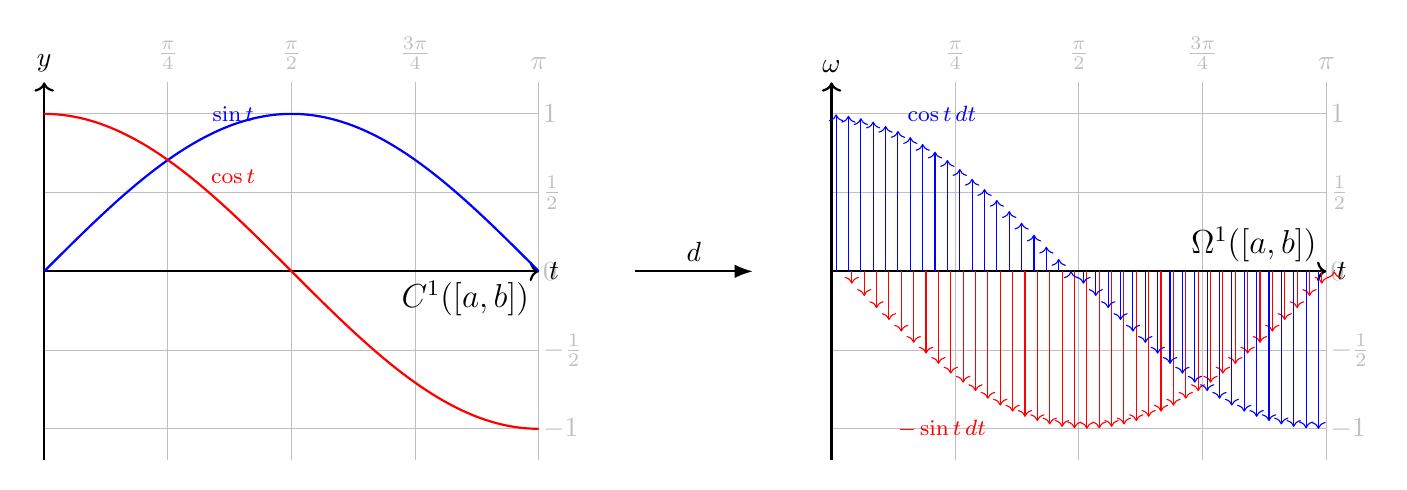
\begin{tikzpicture}[scale=2]
	% numeric constants
	\def\a{0}
	\def\b{3.141592653589793}             % π
	\def\topYmin{0}    \def\topYmax{1.2}
	\def\botYmin{-1.2}\def\botYmax{0}
	
	%── Top panel: C^1([a,b]) ──
	\begin{scope}[]
		% vertical grid lines at t = 0, π/4, π/2, 3π/4, π
		\foreach \x/\xlabel in {
			0.785/{$\tfrac{\pi}{4}$},
			1.570/{$\tfrac{\pi}{2}$},
			2.356/{$\tfrac{3\pi}{4}$},
			3.141/{$\pi$}
		}{
			\draw[lightgray,thin] (\x,-\topYmax) -- (\x,\topYmax)
			node[above,yshift=1pt] {\xlabel};
		}
		% horizontal grid lines at y = 0, 0.5, 1
		\foreach \y/\ylabel in {
			-1/{$-1$},
			-0.5/{$-\tfrac12$},
			0/{$0$},
			0.5/{$\tfrac12$},
			1/{$1$}
		}{
			\draw[lightgray,thin] (\a,\y) -- (\b,\y)
			node[right,xshift=-2pt] {\ylabel};
		}
		% axes
		\draw[->,thick] (\a,\topYmin) -- (\b,\topYmin) node[right] {$t$};
		\draw[->,thick] (\a,-\topYmax) -- (\a,\topYmax) node[above] {$y$};
		% the two C^1–curves
		\draw[blue,thick,domain=\a:\b,samples=200]
		plot (\x,{sin(\x r)});
		\draw[red,thick,domain=\a:\b,samples=200]
		plot (\x,{cos(\x r)});
		% labels
		\node at (\b,0) [below left] {\large $C^1([a,b])$};
		\node[blue] at (1.2,1.0) {\footnotesize$\sin t$};
		\node[red]  at (1.2,0.6) {\footnotesize$\cos t$};
	\end{scope}
	
	%── the exterior derivative arrow ──
	\draw[-Latex, thick] (3.75,0) to node[above] {$d$} (4.5,0);
	
	%── Bottom panel: Ω^1([a,b]) ──
	\begin{scope}[xshift=5cm]
	%── Bottom panel: Ω^1([a,b]) with 11 samples ──
		% grid lines (as before)
		\foreach \x/\xlabel in {
			0.785/{$\tfrac{\pi}{4}$},
			1.570/{$\tfrac{\pi}{2}$},
			2.356/{$\tfrac{3\pi}{4}$},
			3.141/{$\pi$}
		}{
			\draw[lightgray,thin] (\x,-\topYmax) -- (\x,\topYmax)
			node[above,yshift=1pt] {\xlabel};
		}
		% horizontal grid lines at y = 0, 0.5, 1
		\foreach \y/\ylabel in {
			-1/{$-1$},
			-0.5/{$-\tfrac12$},
			0/{$0$},
			0.5/{$\tfrac12$},
			1/{$1$}
		}{
			\draw[lightgray,thin] (\a,\y) -- (\b,\y)
			node[right,xshift=-2pt] {\ylabel};
		}
		% axes
		\draw[->,thick] (\a,0) -- (\b,0) node[right] {$t$};
		\draw[->,thick] (\a,-\topYmax) -- (\a,\topYmax) node[above] {$\omega$};
		
		% sample points t_k = k*pi/10, k=0..10
		\foreach \k in {0.25,0.5,...,10} {
			\pgfmathsetmacro{\x}{\k*pi/10}
			\pgfmathsetmacro{\yone}{cos(\x r)}
			\pgfmathsetmacro{\ytwo}{-sin(\x r)}
			% cos t dt on the left
			\draw[blue,->] ({\x-0.05},0) -- ++(0,{\yone});
			% -sin t dt on the right
			\draw[red,->]  ({\x+0.05},0) -- ++(0,{\ytwo});
		}
		
		% labels
		\node at (\b,\botYmax) [above left] {\large $\Omega^1([a,b])$};
		\node[blue] at (0.7,1) {\footnotesize$\cos t\,dt$};
		\node[red]  at (0.7,-1) {\footnotesize$-\sin t\,dt$};
	\end{scope}
\end{tikzpicture}
\end{center}
The map \[
\fullfunction{d}{C^1([a,b])}{\Omega^1([a,b])}{f(t)}{d(f(t))=df}
\] is defined by $df=f'(t)dt$, where $f'$ is the derivative of $f$. Thus \[
ds:=d(s(t))=s'(t)\; dt=\norm[0]{\gamma'(t)}\; dt.
\]
\end{remark*}
\begin{center}
\begin{minipage}{.5\textwidth}\centering
\includegraphics[scale=1.4]{riemann-tikz/curve_in_3d.pdf}
\end{minipage}\hfill
\begin{minipage}{.49\textwidth}
$\fullfunction{\vec{r}}{\R}{\R^3}{t}{\vec{r}(t)=\gen{x(t),y(t),z(t)}}$\ \\
\vfill\ \\
$\displaystyle\vec{r}'(t)=\frac{d\vec{r}}{dt}
%= \lim_{\Delta t\to0}
%\frac{\gamma(t+\Delta t)-\gamma(t)}{\Delta t}
=\gen{x'(t),y'(t),z'(t)}$\  \\
\vfill\ \\
$\displaystyle s(t)=\int_a^t\norm[0]{\vec{r}'(t)}\; dt$\ \\
$s'(t)=\norm[0]{\vec{r}'(t)}=\sqrt{\left(x'(t)\right)^2+\left(y'(t)\right)^2+\left(z'(t)\right)^2}$\ \\
\ \\
$ds=d(s(t))=s'(t)\; dt=\norm[0]{\vec{r}'(t)}\; dt$
\end{minipage}
\end{center}
\begin{figure}[h!]
\end{figure}
\defbox[Line Integral of Scalar Function over Arc Length]{\begin{definition*}
	Let $f:\R^n\to\R$ be a scalar function, and let $C$ be a piecewise smooth curve in 
$\R^n$ given by a smooth parameterization: \[
\gamma:[a,b]\to\R^n,\quad t\mapsto \gamma(t)=\gen{x_1(t),x_2(t),\dots,x_n(t)}\in\R^n=\operatorname*{dom}(f).
\] The \textbf{line integral of the scalar function} $f$ along the curve $C$ with respect to arc length is defined by \[
\int_C f\; ds :=\int_a^bf(\gamma(t))\norm[0]{\gamma'(t)}\; dt.
\] 
%	Here, $ds=\norm[0]{\gamma'(t)}\; dt$ is the \emph{infinitesimal arc length}.
\end{definition*}}

\newpage
\subsection*{Line Integral of Vector Fields}
\addcontentsline{toc}{subsection}{Line Integral of Vector Fields}
\defbox[Line Integral of a Vector Field in $\R^2$]{\begin{definition*}
Let $C$ be a smooth curve parametrized by \[
\gamma : [a, b] \to \mathbb{R}^2,\quad t\mapsto\gamma(t) = \gen{x(t), y(t)}. 
\] Let \( \mathbf{F} = \gen{F_1, F_2} \) be a smooth vector field on \( \mathbb{R}^2 \).
The \textbf{line integral of the vector field} \( \mathbf{F} \) along the curve \( \gamma \) is defined by \[
\int_C\vec{F}\cdot d\vec{r}=\int_a^b\textbf{F}(\gamma(t))\cdot\gamma'(t)\; dt.
\] Alternatively, \[
\int_C\vec{F}\cdot d\vec{r}=\int_C (F_1,F_2)\cdot(dx,dy)=\int_C F_1dx+F_2dy.
\]
\end{definition*}}

%\thmbox[Fundamental Theorem of Calculus for Line Integrals]{\begin{theorem*}
%Let \(U\subset\mathbb{R}^n\) be open and let \(f\colon U\to\mathbb{R}\) be a \(C^1\)–function. Consider its gradient field by \[
%\nabla f = \gen{\partial_{x_1}f,\dots,\partial_{x_n}f}.
%\] Let \(\gamma\colon[a,b]\to U\) be any piecewise-\(C^1\) curve with endpoints \(\gamma(a)=P\) and \(\gamma(b)=Q\). Then \[
%\int_\gamma \nabla f\cdot d\mathbf r
%\;=\;
%\int_a^b \nabla f\bigl(\gamma(t)\bigr)\cdot\gamma'(t)\,dt
%\;=\;
%f\bigl(\gamma(b)\bigr)\;-\;f\bigl(\gamma(a)\bigr).
%\]

%Exactness.  The condition \(\vec F=\nabla f\) (or \(\omega=df\)) is **necessary and sufficient** for the line integral to depend only on the endpoints of \(\gamma\) and not on its particular shape or parametrization.
%- **Path-Independence.**  Equivalently, in any (piecewise-)connected region on which \(f\) is defined,  
%\[
%\int_{\gamma_1}\nabla f\cdot d\mathbf r
%= 
%\int_{\gamma_2}\nabla f\cdot d\mathbf r
%\]
%whenever \(\gamma_1\) and \(\gamma_2\) share the same start and end points.
%
%Orientation.  Reversing orientation changes the sign:  
%\(\displaystyle\int_{-\gamma}\!\nabla f\cdot d\mathbf r=-\!\int_\gamma\!\nabla f\cdot d\mathbf r.\)
%\end{theorem*}}
%\begin{remark*}[Differential-form version]
%Identify the 1-form  
%	\(\omega = df = \sum_{i=1}^n (\partial_{x^i}f)\,dx^i\).  Then
%	\[
%	\int_\gamma \omega
%	\;=\;
%	\int_a^b \gamma^*\omega
%	\;=\;
%	\int_a^b d\bigl(f\circ\gamma\bigr)
%	\;=\;
%	f\bigl(\gamma(b)\bigr)\;-\;f\bigl(\gamma(a)\bigr).
%	\]
%\end{remark*}

%Excellent — this is a key question for understanding how **vector calculus** connects with **differential forms** and notation. Let's walk through how to **rigorously deduce**:
%
%\[
%\int_C F_1\,dx + F_2\,dy
%\quad \text{from} \quad
%\int_C \vec{F} \cdot d\vec{r}
%\]
%for a vector field \( \vec{F}(x,y) = (F_1(x,y), F_2(x,y)) \).
%
%---
%
%
%
% **Step 1: Parametrize the Curve \( C \)**
%
%Let \( \gamma: [a, b] \to \mathbb{R}^2 \) be a smooth parameterization of the curve \( C \), given by:
%\[
%\gamma(t) = (x(t), y(t)), \quad t \in [a, b].
%\]
%
%Then the **derivative of the curve** is:
%\[
%\gamma'(t) = (x'(t), y'(t)),
%\]
%and the **differential displacement** is:
%\[
%d\vec{r} = \gamma'(t)\,dt = (dx, dy) = (x'(t)\,dt, y'(t)\,dt).
%\]
%
%---
%
% **Step 2: Write the Line Integral of \( \vec{F} \)**
%
%The **vector line integral** is defined as:
%\[
%\int_C \vec{F} \cdot d\vec{r}
%= \int_a^b \vec{F}(\gamma(t)) \cdot \gamma'(t)\,dt
%= \int_a^b \left[ F_1(x(t), y(t))\,x'(t) + F_2(x(t), y(t))\,y'(t) \right] dt.
%\]
%
%---
%
% **Step 3: Recognize the Total Differentials**
%
%From calculus, we know:
%\[
%dx = x'(t)\,dt, \quad dy = y'(t)\,dt.
%\]
%
%Substitute into the integral:
%\[
%\int_a^b F_1(x(t), y(t))\,dx + F_2(x(t), y(t))\,dy.
%\]
%
%So we have:
%\[
%\int_C \vec{F} \cdot d\vec{r}
%= \int_a^b F_1(x(t), y(t))\,dx + F_2(x(t), y(t))\,dy
%= \int_C F_1\,dx + F_2\,dy.
%\]
%
%---
%
%Final Deduction
%
%Thus:
%\[
%\boxed{
%	\int_C \vec{F} \cdot d\vec{r}
%	= \int_C F_1\,dx + F_2\,dy
%}
%\]
%where:
%- \( \vec{F} = (F_1, F_2) \),
%- \( d\vec{r} = (dx, dy) \),
%- The dot product \( \vec{F} \cdot d\vec{r} = F_1\,dx + F_2\,dy \).
%
%---
%
% Interpretation
%
%- The vector line integral becomes an integral of a **1-form**:  
%\[
%\vec{F} \cdot d\vec{r} \quad \leftrightarrow \quad F_1\,dx + F_2\,dy.
%\]
%- The dot product turns into a sum of **components times differentials**.
%
%---
%
%Would you like to go one step further and express this in terms of pullbacks or show how it generalizes to \( \mathbb{R}^3 \)?

%\newpage
%Let \(U\subseteq\mathbb{R}^n\) be an open set and 
%\(\displaystyle\mathbf F:U\to\mathbb{R}^n\) a continuous vector field.  
%Suppose \(C\subset U\) is a smooth curve parametrized by
%\[
%\mathbf r\colon [a,b]\;\longrightarrow\;\mathbb{R}^n,
%\quad
%t\;\mapsto\;\mathbf r(t),
%\]
%with nonzero velocity \(\mathbf r'(t)\).  Then the \emph{line integral} of \(\mathbf F\) along \(C\) is defined by
%\[
%\boxed{
%	\int_C\mathbf F\!\cdot d\mathbf r
%	\;=\;
%	\int_a^b
%	\mathbf F\bigl(\mathbf r(t)\bigr)\;\cdot\;\mathbf r'(t)\;dt
%	\;=\;
%	\int_a^b
%	\sum_{i=1}^n F_i\bigl(\mathbf r(t)\bigr)\,x_i'(t)\;dt,
%}
%\]
%where \(\mathbf r(t)=(x_1(t),\dots,x_n(t))\) and 
%\(\mathbf F=(F_1,\dots,F_n)\).  
%
%\medskip
%
%\noindent
%This integral “accumulates” at each infinitesimal step \(dt\) the projection of \(\mathbf F\) onto the tangent vector \(\mathbf r'(t)\), yielding a single real number that captures the \emph{circulation} or \emph{work} of \(\mathbf F\) along \(C\).
%
%\bigskip
%
%\noindent\textbf{Example.}  Take \(n=2\) and 
%\(\displaystyle \mathbf F(x,y)
%=\Bigl(-\tfrac{y}{x^2+y^2},\,\tfrac{x}{x^2+y^2}\Bigr)\)
%on \(U=\mathbb{R}^2\setminus\{(0,0)\}\).  Let \(C\) be the unit circle 
%\(\;x^2+y^2=1\), counterclockwise.  Parametrize
%\(\mathbf r(t)=(\cos t,\sin t)\), \(t\in[0,2\pi]\).  Then
%\[
%\mathbf r'(t)=(-\sin t,\cos t),\qquad
%\mathbf F\bigl(\mathbf r(t)\bigr)
%=\bigl(-\sin t,\cos t\bigr),
%\]
%so
%\[
%\int_C\mathbf F\!\cdot d\mathbf r
%=\int_0^{2\pi}
%\bigl(-\sin t,\cos t\bigr)\cdot(-\sin t,\cos t)\;dt
%=\int_0^{2\pi}
%\bigl(\sin^2t+\cos^2t\bigr)\;dt
%=2\pi.
%\]
%Thus the total circulation (or “work”) of \(\mathbf F\) around the unit circle is \(2\pi\).


\paragraph{{\color{magenta}Problem\;\#1} (Line Integral around Unit Circle).} Let \( C \subset \mathbb{R}^2 \) be the unit circle defined by $
C: x^2 + y^2 = 1,$ traversed in the \emph{counterclockwise direction}. Let the vector field \( \vec{F}: \mathbb{R}^2 \setminus \{(0,0)\} \to \mathbb{R}^2 \) be defined by \[
\vec{F}(x, y) = \Gen{\frac{-y}{x^2 + y^2},\; \frac{x}{x^2 + y^2} }.
\] Evaluate the \emph{line integral} of \( \vec{F} \) along \( C \): \[
\oint_C \vec{F} \cdot d\vec{r}.
\]
\begin{proof}[\sol]
\ \begin{center}
\begin{minipage}{.49\textwidth}\centering
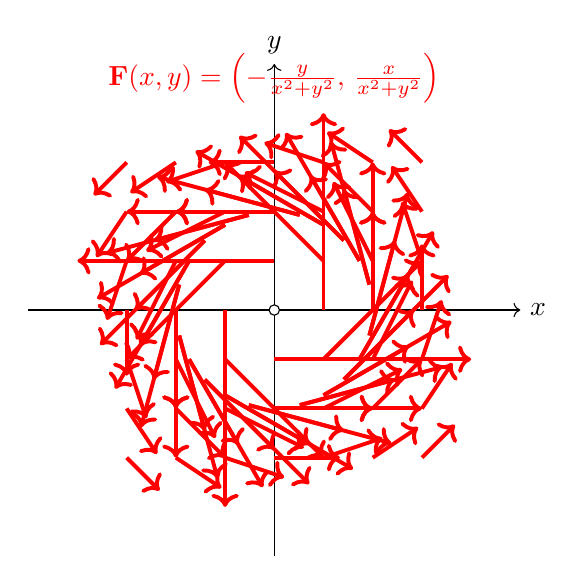
\begin{tikzpicture}[scale=1.25]
%	\draw[dashed, gray!20] (-4,-4) grid (4,4);
	% Axes
	\draw[->] (-2.5,0) -- (2.5,0) node[right] {$x$};
	\draw[->] (0,-2.5) -- (0,2.5) node[above] {$y$};
	% Desired arrow length
	\def\arrowlen{1}	
	% Loop over integer grid points
	\foreach \X in {-1.5,-1,-.5,0,.5,1,1.5} {
		\foreach \Y in {-1.5,-1,-.5,0,.5,1,1.5} {
			% Compute radius r = sqrt(x^2+y^2)
			\pgfmathsetmacro{\r}{\X*\X + \Y*\Y}
			
			\ifdim \r pt=0pt
			% At (0,0): singularity
			\fill[white,draw=black] (0,0) circle (1.5pt);
			\else
			% Compute unit‐tangent components then scale
			\pgfmathsetmacro{\dx}{(-\Y/\r)*\arrowlen}
			\pgfmathsetmacro{\dy}{(\X/\r)*\arrowlen}
			
			% Draw the arrow
			\draw[->, line width=.5mm, red]
			(\X,\Y) -- ++(\dx,\dy);
			\fi
		}
	}
	\foreach \t in {0,15,...,345}{
		\pgfmathsetmacro\x{cos(\t)}
		\pgfmathsetmacro\y{sin(\t)}
		% On r=1, F = (-y,x)
		\pgfmathsetmacro\dx{(-\y)*\arrowlen}
		\pgfmathsetmacro\dy{(\x)*\arrowlen}
		\draw[->, line width=.5mm, red] 
		(\x,\y) -- ++(\dx,\dy);
	}
	\def\arrowlen{1.5}
	\foreach \t in {0,15,...,345}{
		\pgfmathsetmacro\x{cos(\t)}
		\pgfmathsetmacro\y{sin(\t)}
		% On r=1, F = (-y,x)
		\pgfmathsetmacro\dx{(-\y)*\arrowlen}
		\pgfmathsetmacro\dy{(\x)*\arrowlen}
		\draw[->, line width=.5mm, red] 
		(\x,\y) -- ++(\dx,\dy);
	}
	
	%--- Annotations -----------------------------------------
	\node[above, red] at (0,2)
	{$\vec{F}(x,y)=\left(-\tfrac{y}{x^2+y^2},\,\tfrac{x}{x^2+y^2}\right)$};
\end{tikzpicture}
\end{minipage}
\begin{minipage}{.49\textwidth}\centering
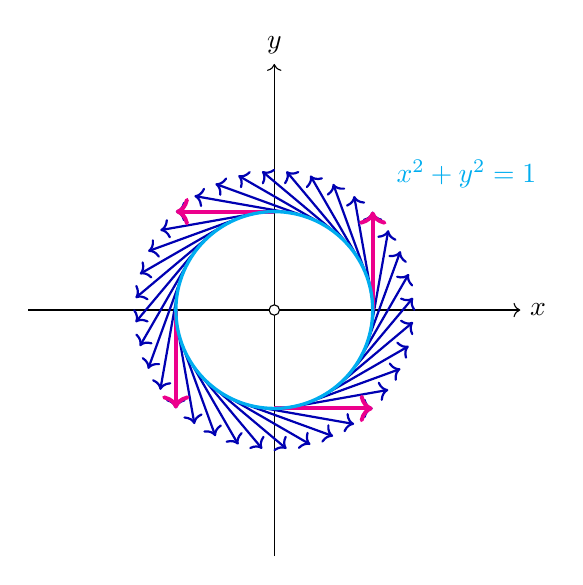
\begin{tikzpicture}[scale=1.25]
	%	\draw[dashed, gray!20] (-4,-4) grid (4,4);
	% Axes
	\draw[->] (-2.5,0) -- (2.5,0) node[right] {$x$};
	\draw[->] (0,-2.5) -- (0,2.5) node[above] {$y$};
	\fill[white,draw=black] (0,0) circle (1.5pt);
	\def\arrowlen{1}
	\foreach \t in {0,10,...,350}{
		\pgfmathsetmacro\x{cos(\t)}
		\pgfmathsetmacro\y{sin(\t)}
		% On r=1, F = (-y,x)
		\pgfmathsetmacro\dx{(-\y)*\arrowlen}
		\pgfmathsetmacro\dy{(\x)*\arrowlen}
		\draw[->, thick, blue!70!black] 
		(\x,\y) -- ++(\dx,\dy);
	}
	\foreach \t in {0,90,180,270}{
		\pgfmathsetmacro\x{cos(\t)}
		\pgfmathsetmacro\y{sin(\t)}
		% On r=1, F = (-y,x)
		\pgfmathsetmacro\dx{(-\y)*\arrowlen}
		\pgfmathsetmacro\dy{(\x)*\arrowlen}
		\draw[->, line width=.5mm, magenta] 
		(\x,\y) -- ++(\dx,\dy);
	}
	%--- Draw contour C with orientation --------------------
	\draw[cyan, very thick]
	(0,0) circle (1)
	node[above right=2cm] {$x^2+y^2=1$};
\end{tikzpicture}
\end{minipage}
\end{center}
%\begin{tikzpicture}[scale=1.5]
%	% Axes
%	\draw[->] (-2.5,0) -- (2.5,0) node[right] {$x$};
%	\draw[->] (0,-2.5) -- (0,2.5) node[above] {$y$};
%	
%	% The unit circle
%	\draw[cyan, very thick] (0,0) circle (1) node[above right=2cm] {$x^2+y^2=1$};
%	
%	% Tangential field F = (-y,x)
%	\def\arrowlen{1}
%	\foreach \t in {0,10,...,350}{
%		\pgfmathsetmacro\x{cos(\t)}
%		\pgfmathsetmacro\y{sin(\t)}
%		\pgfmathsetmacro\dx{(-\y)*\arrowlen}
%		\pgfmathsetmacro\dy{(\x)*\arrowlen}
%		\draw[->, thick, blue!70!black] (\x,\y) -- ++(\dx,\dy);
%	}
%	
%	% Highlight four sample vectors thicker
%	\foreach \t in {0,90,180,270}{
%		\pgfmathsetmacro\x{cos(\t)}
%		\pgfmathsetmacro\y{sin(\t)}
%		\draw[->, line width=.5mm, magenta] 
%		(\x,\y) -- ++(-\y,\x);
%	}
%	
%	% Annotate that curl F = 0 off the origin
%	\node[red] at (1.5,1.5) {\small$\displaystyle\nabla\times\mathbf F = 0$};
%	\filldraw[red] (0,0) circle(1.5pt) node[below right=2pt] 
%	{\small “hole” at $(0,0)$};
%\end{tikzpicture}
\newpage\noindent
Consider the vector field $
\vec{F}(x, y) = \Gen{\frac{-y}{x^2 + y^2},\; \frac{x}{x^2 + y^2}}$,
and the curve \( C \) is the unit circle \( x^2 + y^2 = 1 \), traversed counterclockwise.
%\begin{enumerate}[\bfseries Step 1.]
%	\item 
\ \\
	\textbf{(Parametrization)} Define a function \[
	\fullfunction{\gamma}{[0,2\pi]}{\set{(x,y)\in\R^2:x^2+y^2=1}}{\theta}{\gamma(\theta)=(\cos\theta,\sin\theta)}.
	\] Here, $\frac{d\gamma}{d\theta}=(-\sin\theta,\cos\theta)$.
	\begin{center}
	\begin{minipage}{.4\textwidth}\centering
	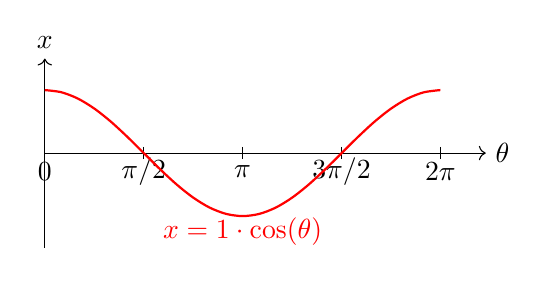
\begin{tikzpicture}[scale=.8]
		% Draw axes
		\draw[->] (0,-1.5) -- (0,1.5) node[above] {\(x\)};
		\draw[->] (0,0) -- (7,0) node[right] {\(\theta\)};
		
		% Mark key points on the t-axis (0, pi/2, pi, 3pi/2, 2pi)
		\foreach \x in {0,1.57,3.14,4.71,6.28} {
			\draw (\x,0.1) -- (\x,-0.1);
		}
		\node at (0,-0.3) {\(0\)};
		\node at (1.57,-0.3) {\(\pi/2\)};
		\node at (3.14,-0.3) {\(\pi\)};
		\node at (4.71,-0.3) {\(3\pi/2\)};
		\node at (6.28,-0.3) {\(2\pi\)};
		
		% Draw sin(t) in blue
	%	\draw[domain=0:6.28, smooth, variable=\t, blue, thick] 
	%	plot ({\t},{sin(\t r)});
	%	\node[blue] at (1.67,1.25) {\(\sin(t)\)};
		
		% Draw cos(t) in red
		\draw[domain=0:6.28, smooth, variable=\t, red, thick] 
		plot ({\t},{cos(\t r)});
		\node[red] at (3.14,-1.25) {\(x=1\cdot\cos(\theta)\)};
	\end{tikzpicture}
	\end{minipage}\hfill
	\begin{minipage}{.4\textwidth}\centering
	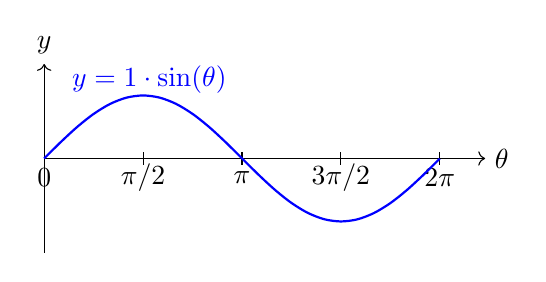
\begin{tikzpicture}[scale=.8]
		% Draw axes
		\draw[->] (0,-1.5) -- (0,1.5) node[above] {\(y\)};
		\draw[->] (0,0) -- (7,0) node[right] {\(\theta\)};
		
		% Mark key points on the t-axis (0, pi/2, pi, 3pi/2, 2pi)
		\foreach \x in {0,1.57,3.14,4.71,6.28} {
			\draw (\x,0.1) -- (\x,-0.1);
		}
		\node at (0,-0.3) {\(0\)};
		\node at (1.57,-0.3) {\(\pi/2\)};
		\node at (3.14,-0.3) {\(\pi\)};
		\node at (4.71,-0.3) {\(3\pi/2\)};
		\node at (6.28,-0.3) {\(2\pi\)};
		
		% Draw sin(t) in blue
		\draw[domain=0:6.28, smooth, variable=\t, blue, thick] 
		plot ({\t},{sin(\t r)});
		\node[blue] at (1.67,1.25) {\(y=1\cdot \sin(\theta)\)};
		
		% Draw cos(t) in red
	%	\draw[domain=0:6.28, smooth, variable=\t, red, thick] 
	%	plot ({\t},{cos(\t r)});
	%	\node[red] at (3.14,-1.25) {\(\cos(t)\)};
	\end{tikzpicture}
	\end{minipage}
	\end{center}
%	\item 
	\textbf{(Evaluate $\textbf{F}(\gamma(\theta))$ and the dot product)}\; We have \[
	\vec{F}(\gamma(\theta)) = \vec{F}(\cos\theta,\sin\theta) \overset{\sin^2\theta+\cos^2\theta=1}{=} \Gen{\frac{-\sin \theta}{1}, \frac{\cos \theta}{1} }
	= (-\sin \theta, \cos \theta).
	\] and \[
	\vec{F}(\gamma(\theta)) \cdot \frac{d\gamma}{d\theta}
	= (-\sin \theta)(-\sin \theta) + (\cos \theta)(\cos \theta)
	= \sin^2 \theta + \cos^2 \theta = 1.
	\]
%	\item 
	\textbf{(Integral)} \[
	\oint_C \vec{F} \cdot d\vec{r}
	= \int_0^{2\pi} \vec{F}(\gamma(\theta)) \cdot\frac{d\gamma}{d\theta}\,d\theta
	= \int_0^{2\pi} 1\,d\theta = 2\pi.
	\]
%\end{enumerate}
\end{proof}

\newpage
\section*{Surface Integral for Vector Fields}
\addcontentsline{toc}{section}{Surface Integral for Vector Fields}
%\defbox[Surface Integral of a Vector Field]{\begin{definition*}
%Let \(S\subset\mathbb{R}^3\) be a smooth, oriented surface, and let  
%	\[
%	T\colon D\;\subseteq\;\mathbb{R}^2\;\longrightarrow\;S,
%	\qquad
%	(u,v)\;\longmapsto\;T(u,v),
%	\]  
%	be a regular \(C^1\) parametrization whose orientation agrees with that of \(S\).  Consider the partial‐derivative (tangent) vectors \[
%	T_u(u,v)=\frac{\partial T}{\partial u}(u,v),
%	\quad
%	T_v(u,v)=\frac{\partial T}{\partial v}(u,v),
%	\]  and the induced normal‐vector field  
%	\[
%	N(u,v)\;=\;T_u(u,v)\times T_v(u,v)\;\in\;\mathbb{R}^3,
%	\]  
%	which is everywhere nonzero on \(D\) and points according to the chosen orientation.
%	Now let  \[
%	\mathbf F\colon U\;(\supseteq S)\;\longrightarrow\;\mathbb{R}^3
%	\]  
%	be a continuous (or \(C^1\)) vector field defined on an open neighborhood \(U\) of \(S\).  Then \textbf{the surface integral of \(\mathbf F\) over \(S\)} is defined by the formula  
%	\[
%	\boxed{
%		\iint_{S} \mathbf F\;\cdot\;d\mathbf S
%		\;=\;
%		\iint_{D}
%		\mathbf F\bigl(T(u,v)\bigr)\;\cdot\;N(u,v)
%		\;du\,dv
%		\;=\;
%		\iint_{D}
%		\mathbf F\bigl(T(u,v)\bigr)\;\cdot\;
%		\bigl(T_u(u,v)\times T_v(u,v)\bigr)
%		\;du\,dv.
%	}
%	\]
%\end{definition*}}
%\begin{remark*}
%	1. **Geometric meaning.**  
%	At each point \(T(u,v)\in S\), the vector \(N(u,v)\,du\,dv\) represents the oriented area element \(d\mathbf S\).  Thus \(\mathbf F\cdot d\mathbf S\) measures how much \(\mathbf F\) “flows through” that little patch of surface.
%	
%	2. **Independence of parametrization.**  
%	If \(\widetilde T\colon \widetilde D\to S\) is any other orientation‐preserving \(C^1\) parametrization, then a change‐of‐variables argument shows  
%	\[
%	\iint_{D}\mathbf F\cdot\bigl(T_u\times T_v\bigr)\,du\,dv
%	\;=\;
%	\iint_{\widetilde D}\mathbf F\cdot\bigl(\widetilde T_u\times\widetilde T_v\bigr)\,d\widetilde u\,d\widetilde v.
%	\]
%	
%	3. **Special case (scalar area).**  
%	Taking \(\mathbf F=(0,0,1)\) recovers the usual surface‐area integral  
%	\(\displaystyle \mathrm{Area}(S)=\iint_S dS=\iint_D\|T_u\times T_v\|\,du\,dv.\)
%	
%	This definition is the standard one found in graduate‐level treatments of differential geometry and vector calculus.
%\end{remark*}

\paragraph{{\color{magenta}Problem\;\#2} (Surface‐Flux).} Compute the surface integral
\[
\iint_{S} \mathbf{F}\,\cdot\,d\mathbf{S},
\]
where $\mathbf{F}(x,y,z)
= \langle x,\;y,\;-z\rangle$ and the surface \(S\) is parametrized by \[
\mathbf{r}(u,v) 
= \langle u + 2v,\;2u + v,\;3uv\rangle,
\quad (u,v)\in[0,1]\times[0,1].
\]
\begin{proof}[\sol]
%\ \begin{center}
%\begin{minipage}{.475\textwidth}\centering
%	\includegraphics[width=.75\textwidth]{riemann-tikz/problem2_1.pdf}
%\end{minipage}\hfill
%\begin{minipage}{.475\textwidth}\centering
%	\includegraphics[width=.75\textwidth]{riemann-tikz/problem2_2_2.pdf}
%\end{minipage}
%\end{center}
\ \begin{enumerate}[\bfseries 1.]
	\item \textbf{Parametrization and partials.\;} The surface is  
	\[
	S=\mathbf r\bigl([0,1]^2\bigr),
	\qquad
	\mathbf r(u,v)=(\,u+2v,\;2u+v,\;3uv\,),
	\]
	and then \[
	\mathbf{r}_u = \frac{\partial\mathbf{r}}{\partial u}
	= \langle 1,\,2,\,3v\rangle,
	\quad
	\mathbf{r}_v = \frac{\partial\mathbf{r}}{\partial v}
	= \langle 2,\,1,\,3u\rangle.
	\]
	\begin{center}
	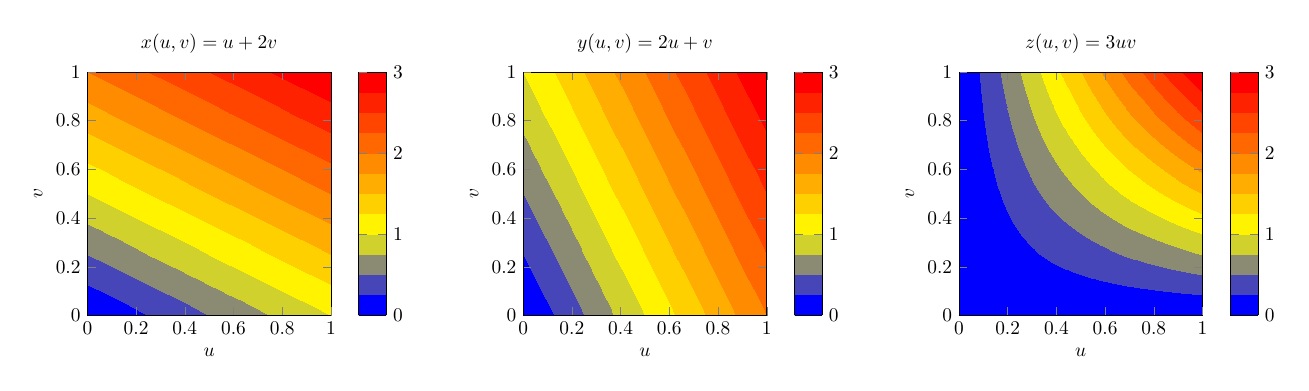
\begin{tikzpicture}[scale=.7]
		\begin{axis}[
			name=plot1,
			title={$x(u,v) = u+2v$},
			xlabel={$u$}, ylabel={$v$},
			width=6cm, height=6cm,
			view={0}{90}, % Top-down 2D view
			colorbar
			]
			\addplot3[
			contour filled={number=12},
			domain=0:1, y domain=0:1
			] {x + 2*y};
		\end{axis}
		
		\begin{axis}[
			at=(plot1.right of east), anchor=left of west, xshift=2.2cm,
			name=plot2,
			title={$y(u,v) = 2u+v$},
			xlabel={$u$}, ylabel={$v$},
			width=6cm, height=6cm,
			view={0}{90},
			colorbar
			]
			\addplot3[
			contour filled={number=12},
			domain=0:1, y domain=0:1
			] {2*x + y};
		\end{axis}
		
		\begin{axis}[
			at=(plot2.right of east), anchor=left of west, xshift=2.2cm,
			title={$z(u,v) = 3uv$},
			xlabel={$u$}, ylabel={$v$},
			width=6cm, height=6cm,
			view={0}{90},
			colorbar
			]
			\addplot3[
			contour filled={number=12},
			domain=0:1, y domain=0:1
			] {3*x*y};
		\end{axis}
	\end{tikzpicture}
	\end{center}
	\begin{center}
%	\begin{tikzpicture}[scale=.7]
%		\begin{axis}[
%			name=plotA,
%			title={Surface Colored by $x=u+2v$},
%			xlabel={$x$}, ylabel={$y$}, zlabel={$z$},
%			view={185}{30}, colorbar,
%			width=6cm, height=6cm,			
%			xmax=2, ymax=2, zmax=1.5,
%			]
%			\addplot3[
%			surf, domain=0:1, y domain=0:1,
%			variable=\u, variable y=\v,
%			point meta={\u+2*\v} % Color by x-value
%			]
%			({u + 2*v}, {2*u + v}, {3*u*v});
%		\end{axis}
%		
%		\begin{axis}[
%			at=(plotA.right of east), anchor=left of west, xshift=2.2cm,
%			name=plotB,
%			title={Surface Colored by $y=2u+v$},
%			xlabel={$x$}, ylabel={$y$}, zlabel={$z$},
%			view={95}{30}, colorbar,
%			width=6cm, height=6cm,			
%			xmax=2, ymax=2, zmax=1.5,
%			]
%			\addplot3[
%			surf, domain=0:1, y domain=0:1,
%			variable=\u, variable y=\v,
%			point meta={2*\u+\v} % Color by y-value
%			]
%			({u + 2*v}, {2*u + v}, {3*u*v});
%		\end{axis}
%		
%		\begin{axis}[
%			at=(plotB.right of east), anchor=left of west, xshift=2.2cm,
%			title={Surface Colored by $z=3uv$},
%			xlabel={$x$}, ylabel={$y$}, zlabel={$z$},
%			view={125}{30}, colorbar,
%			width=6cm, height=6cm	,		
%			xmax=2, ymax=2, zmax=1.5,
%			]
%			\addplot3[
%			surf, domain=0:1, y domain=0:1,
%			variable=\u, variable y=\v,
%			point meta={3*\u*\v} % Color by z-value
%			]
%			({u + 2*v}, {2*u + v}, {3*u*v});
%		\end{axis}
%	\end{tikzpicture}
	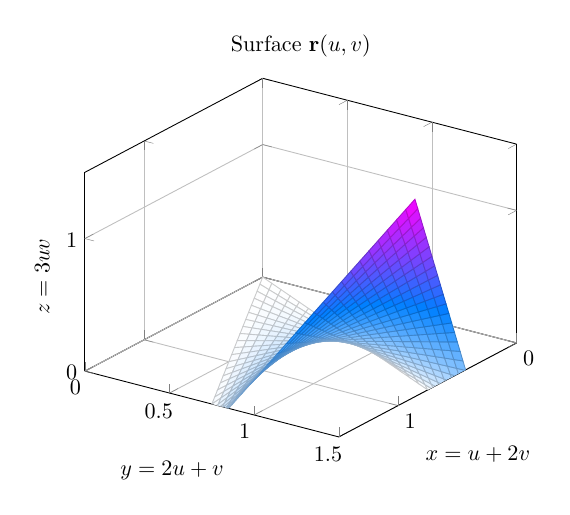
\begin{tikzpicture}[scale=.8]
		\begin{axis}[
			title={Surface $\mathbf{r}(u,v)$},
			xlabel={$x = u+2v$},
			ylabel={$y = 2u+v$},
			zlabel={$z = 3uv$},
			view={125}{30}, % Viewing angle
			xmin=0, ymin=0, zmin=0, % Set axis limits
			xmax=1.5, ymax=1.5, zmax=1.5,
			grid=major,
%			colormap/viridis
			colormap/cool
			]
			\addplot3[
			surf,
			domain=0:1,         % u-range
			y domain=0:1,       % v-range
			samples=25,         % #sample
			variable=\u,        % domain
			variable y=\v,      % co-domain
			]
			({u + 2*v}, {2*u + v}, {3*u*v});
		\end{axis}
	\end{tikzpicture}
	\end{center}
	\item \textbf{Oriented normal.\;} The induced normal vector is the cross‐product
	\begin{align*}
		\mathbf r_u\times \mathbf r_v
		&=\det\begin{vmatrix}
			\mathbf i & \mathbf j & \mathbf k\\
			1 & 2 & 3v\\
			2 & 1 & 3u
		\end{vmatrix}\\
		&=\det\begin{vmatrix}
			2 & 3v \\ 1 & 3u
		\end{vmatrix}\textbf{i}-
		\det\begin{vmatrix}
			1 & 3v \\ 2 & 3u
		\end{vmatrix}\textbf{j}+
		\det\begin{vmatrix}
			1 & 2 \\ 2 & 1
		\end{vmatrix}\textbf{k}
		\\
		&=\bigl\langle 6u - 3v,\; -3u + 6v,\; -3 \bigr\rangle.
	\end{align*}
\end{enumerate}


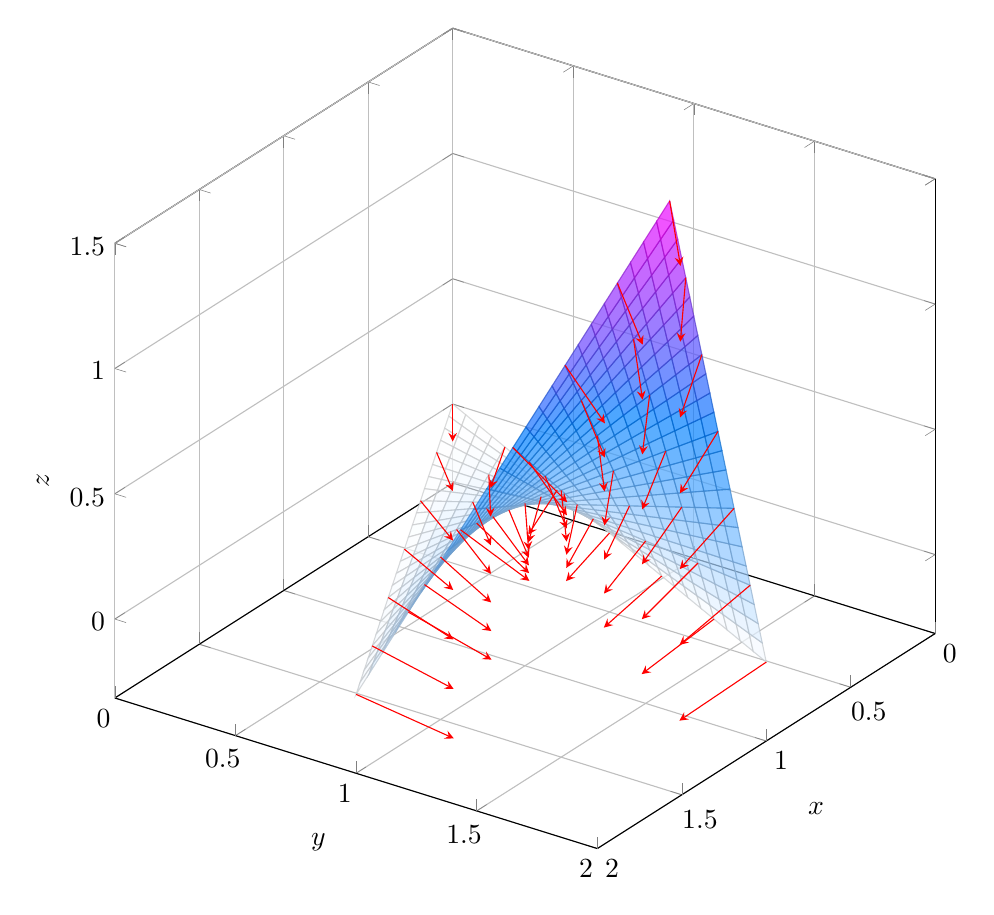
\begin{tikzpicture}[scale=1]
	\begin{axis}[
%		title={Surface with Normal Vector Field $\mathbf{r}_u \times \mathbf{r}_v$},
		xlabel={$x$},
		ylabel={$y$},
		zlabel={$z$},
		view={125}{30}, % Set a good viewing angle
		grid=major,
		width=12cm,
		height=12cm,
		xmax=2, ymax=2, zmax=1.5,
		z buffer=sort  % Ensures correct 3D layering
		]
		% 1. Plot the surface (semi-transparent)
		\addplot3[
		surf,
		domain=0:1,
		y domain=0:1,
		samples=25,
		variable=\u,
		variable y=\v,
		colormap/cool,
		opacity=0.7
		]
		({u + 2*v}, {2*u + v}, {3*u*v});
		
		% 2. Plot the normal vector field using quiver
		\addplot3[
		-stealth, % Adds arrowheads
		red,
		samples=7, % Creates a 7x7 grid of vectors
		domain=0:1,
		y domain=0:1,
		variable=\u,
		variable y=\v,
		quiver={
			% Vector components (u,v,w) for the direction
			u={6*u - 3*v},
			v={-3*u + 6*v},
			w={-3},
			scale arrows=0.05 % Adjusts arrow length for visibility
		}
		]
		% Base point (x,y,z) for each vector
		({u + 2*v}, {2*u + v}, {3*u*v});
	\end{axis}
\end{tikzpicture}

\subsection*{Detailed Justification for \(\mathbf r_u\times\mathbf r_v\) as Surface Normal}

Let 
\[
\mathbf r(u,v)=(\,x(u,v),\,y(u,v),\,z(u,v)\,)
\]
be a smooth parametrization of a surface patch \(S\subset\R^3\).  Then at each point \((u,v)\), the two tangent vectors
\[
\mathbf r_u
=\frac{\partial\mathbf r}{\partial u}
\quad\text{and}\quad
\mathbf r_v
=\frac{\partial\mathbf r}{\partial v}
\]
span the tangent plane to \(S\).  We list the logical steps that show
\(\mathbf r_u\times\mathbf r_v\)
is the correct (non-unit) normal vector:

\begin{enumerate}
	\item \textbf{Tangent plane.}  By definition of partial derivatives,
	\[
	\mathbf r_u\;\text{is the velocity of the curve }v=\text{const},
	\quad
	\mathbf r_v\;\text{is the velocity of the curve }u=\text{const}.
	\]
	Both lie tangent to the surface.
	
	\item \textbf{Cross product properties.}  In \(\R^3\), the cross product 
	\(\mathbf a\times\mathbf b\) satisfies:
	\[
	\mathbf a\times\mathbf b
	\perp \mathbf a,
	\quad
	\mathbf a\times\mathbf b
	\perp \mathbf b,
	\]
	and its direction is given by the right-hand rule (orientation of \((\mathbf a,\mathbf b,\mathbf a\times\mathbf b)\)).  Thus
	\(\mathbf r_u\times\mathbf r_v\)
	is perpendicular to the tangent plane.
	
	\item \textbf{Determinant formula.}  One defines
	\[
	\mathbf a\times\mathbf b
	= \det
	\begin{pmatrix}
		\mathbf i & \mathbf j & \mathbf k\\
		a_1        & a_2        & a_3\\
		b_1        & b_2        & b_3
	\end{pmatrix},
	\]
	which expands by minors to give the familiar component formula
	\(\bigl(a_2b_3 - a_3b_2,\; a_3b_1 - a_1b_3,\;a_1b_2 - a_2b_1\bigr)\).
	
	\item \textbf{Application to our \(\mathbf r_u,\mathbf r_v\).}  
	In our case,
	\[
	\mathbf r_u=\langle 1,\,2,\,3v\rangle,
	\quad
	\mathbf r_v=\langle 2,\,1,\,3u\rangle.
	\]
	Plugging into the determinant formula yields
	\[
	\mathbf r_u\times\mathbf r_v
	= 
	\begin{vmatrix}
		\mathbf i & \mathbf j & \mathbf k\\
		1         & 2         & 3v      \\
		2         & 1         & 3u
	\end{vmatrix}
	= \bigl\langle 2\cdot3u-3v\cdot1,\;- (1\cdot3u-3v\cdot2),\;1\cdot1-2\cdot2\bigr\rangle
	=\langle 6u-3v,\;-3u+6v,\;-3\rangle.
	\]
	
	\item \textbf{Verification of orthogonality.}  One can check directly
	\[
	(\mathbf r_u\times\mathbf r_v)\;\cdot\;\mathbf r_u
	=0,
	\quad
	(\mathbf r_u\times\mathbf r_v)\;\cdot\;\mathbf r_v
	=0,
	\]
	confirming it is indeed normal.
	
	\item \textbf{Geometric interpretation.}  The magnitude
	\(\|\mathbf r_u\times\mathbf r_v\|\) equals the area of the parallelogram spanned by \(\mathbf r_u,\mathbf r_v\).  Thus in surface integrals
	\(\iint_S \mathbf F\cdot d\mathbf S\), one uses
	\(\mathbf r_u\times\mathbf r_v\,du\,dv\) as the oriented area element.
	
\end{enumerate}

\noindent In summary, the cross‐product of the partial derivatives is the unique algebraic construction in \(\R^3\) that (i) is bilinear and alternating, (ii) yields a vector orthogonal to both inputs, and (iii) has magnitude equal to the parallelogram area—exactly capturing the normal and area element needed for surface integrals.

\section*{The Cross Product in \(\R^3\)}

\subsection*{Definition}
For two vectors
\[
\mathbf u = (u_1,u_2,u_3),
\qquad
\mathbf v = (v_1,v_2,v_3)
\]
in \(\R^3\), their \emph{cross product} \(\mathbf u \times \mathbf v\) is defined to be the vector
\[
\mathbf u \times \mathbf v
=
\bigl(
u_2v_3 - u_3v_2,\;
u_3v_1 - u_1v_3,\;
u_1v_2 - u_2v_1
\bigr).
\]
Equivalently, if \((\mathbf e_1,\mathbf e_2,\mathbf e_3)\) is the standard basis, one writes formally
\[
\mathbf u \times \mathbf v
= 
\begin{vmatrix}
	\mathbf e_1 & \mathbf e_2 & \mathbf e_3\\
	u_1         & u_2         & u_3         \\
	v_1         & v_2         & v_3
\end{vmatrix},
\]
meaning “take the determinant by expanding along the first row.”

\subsection*{Key Properties}
\begin{enumerate}
	\item \textbf{Bilinearity and Alternation:}
	\(\mathbf u\times(\mathbf v+\mathbf w)
	=\mathbf u\times\mathbf v
	+\mathbf u\times\mathbf w,\)
	and
	\(\mathbf u\times\mathbf v = -\,(\mathbf v\times\mathbf u).\)
	
	\item \textbf{Perpendicularity:}
	\(\mathbf u\times\mathbf v\) is orthogonal to both \(\mathbf u\) and \(\mathbf v\):
	\(\;(\mathbf u\times\mathbf v)\cdot\mathbf u=0\),
	\((\mathbf u\times\mathbf v)\cdot\mathbf v=0.\)
	
	\item \textbf{Magnitude = Area:}
	\[
	\|\mathbf u\times\mathbf v\|
	= \|\mathbf u\|\,\|\mathbf v\|\;\bigl|\sin\theta\bigr|
	= \text{area of the parallelogram spanned by \(\mathbf u,\mathbf v\)},
	\]
	where \(\theta\) is the angle between \(\mathbf u\) and \(\mathbf v\).
	
	\item \textbf{Right‐Hand Rule (Orientation):}
	The triple \((\mathbf u,\mathbf v,\mathbf u\times\mathbf v)\) has the same “right‐hand” orientation as the standard basis \((\mathbf e_1,\mathbf e_2,\mathbf e_3)\).
\end{enumerate}

\subsection*{Why the Determinant Formula?}

The determinant expression
\[
\mathbf u\times\mathbf v
=\det
\begin{pmatrix}
	\mathbf e_1 & \mathbf e_2 & \mathbf e_3\\
	u_1         & u_2         & u_3         \\
	v_1         & v_2         & v_3
\end{pmatrix}
\]
is not a literal \(3\times3\) determinant of numbers, but a \emph{mnemonic} encoding exactly those three component‐wise minors which satisfy:

\begin{itemize}
	\item \emph{Alternation:} Swapping the two rows \((u_i)\) and \((v_i)\) changes the sign of each minor, matching \(\mathbf v\times\mathbf u=-(\mathbf u\times\mathbf v)\).
	\item \emph{Bilinearity:} Expanding a determinant along the top row is linear in each column.
	\item \emph{Compatibility with basis:} For the standard basis vectors,
	\[
	\mathbf e_1\times\mathbf e_2 = \mathbf e_3,\quad
	\mathbf e_2\times\mathbf e_3 = \mathbf e_1,\quad
	\mathbf e_3\times\mathbf e_1 = \mathbf e_2,
	\]
	and all others follow by bilinearity and alternation.
\end{itemize}

Concretely, expanding along the first row gives
\begin{align*}
	\mathbf r_u \times \mathbf r_v
	&=
	\det
	\begin{pmatrix}
		\mathbf i & \mathbf j & \mathbf k\\
		1         & 2         & 3v\\
		2         & 1         & 3u
	\end{pmatrix}\\
	&=
	\mathbf i\,(2\cdot3u - 1\cdot3v)
	-
	\mathbf j\,(1\cdot3u - 2\cdot3v)
	+
	\mathbf k\,(1\cdot1   - 2\cdot2)\\
	&=
	\bigl\langle 6u - 3v,\;-3u + 6v,\;-3\bigr\rangle.
\end{align*}

which reproduces the component‐wise definition above.

\subsection*{Geometric Interpretation via Volumes}

Another way to see the determinant is to note that in \(\R^3\) the scalar triple product
\(\det[\mathbf u,\mathbf v,\mathbf w]\)
gives the signed volume of the parallelepiped spanned by \(\mathbf u,\mathbf v,\mathbf w\).  If one fixes \(\mathbf u,\mathbf v\), then the unique vector \(\mathbf n\) satisfying
\[
\det[\mathbf u,\mathbf v,\mathbf n] = \|\mathbf u\times\mathbf v\|^2
\quad\text{and}\quad
\mathbf n\perp \mathbf u,\mathbf v
\]
is precisely \(\mathbf u\times\mathbf v\).  The determinant‐of‐a‐matrix formula encodes that same volume‐and‐orientation condition intrinsically.

\bigskip

\noindent\emph{Conclusion:}  The cross product is the unique bilinear, alternating, oriented map \(\R^3\times\R^3\to\R^3\) whose length measures area; the \(3\times3\) “determinant” notation succinctly packages its component formula and all of its key properties in one place.









2. **

3. **Pullback of the field.**  
The given field is \(\mathbf F(x,y,z)=(x,y,-z)\).  Along the patch,
\[
\mathbf F\bigl(\mathbf r(u,v)\bigr)
=\bigl(u+2v,\;2u+v,\;-3uv\bigr).
\]

4. **Integrand.**  
Taking the dot‐product,
\begin{align*}
	\mathbf F(\mathbf r)\,\cdot\,(\mathbf r_u\times\mathbf r_v)
	&= (u+2v)(6u-3v)\;+\;(2u+v)(-3u+6v)\;+\;(-3uv)(-3)\\
	&= 6u^2 -3uv +12uv -6v^2 \;-\;6u^2 +12uv -3uv +6v^2 \;+\;9uv\\
	&=(-3uv+12uv+12uv-3uv+9uv)\;=\;27\,u\,v.
\end{align*}

5. **Double integral.**  
Thus the flux is
\[
\iint_{S}\mathbf F\cdot d\mathbf S
\;=\;
\iint_{[0,1]^2}27\,u\,v\;du\,dv
\;=\;
27\int_0^1\!\int_0^1 u\,v\;du\,dv
\;=\;
27\Bigl(\tfrac12\Bigr)\Bigl(\tfrac12\Bigr)
\;=\;\frac{27}{4}.
\]

Hence  
\[
\boxed{\iint_{S}\mathbf F\cdot d\mathbf S \;=\;\frac{27}{4}}.
\]

\newpage
\begin{enumerate}
	\item Compute the partial derivatives:
	\[
	\mathbf{r}_u = \frac{\partial\mathbf{r}}{\partial u}
	= \langle 1,\,2,\,3v\rangle,
	\quad
	\mathbf{r}_v = \frac{\partial\mathbf{r}}{\partial v}
	= \langle 2,\,1,\,3u\rangle.
	\]
	\item Form the cross‑product to get the oriented area element:
	\[
	\mathbf{r}_u\times\mathbf{r}_v
	= 
	\begin{vmatrix}
		\mathbf{i} & \mathbf{j} & \mathbf{k} \\
		1 & 2 & 3v \\
		2 & 1 & 3u
	\end{vmatrix}
	= \bigl\langle 6u - 3v,\; -3u + 6v,\; -3 \bigr\rangle.
	\]
	Hence
	\[
	d\mathbf{S}
	= \bigl(\mathbf{r}_u \times \mathbf{r}_v\bigr)\,du\,dv.
	\]
	\item Evaluate \(\mathbf{F}\) on the parametrization:
	\[
	\mathbf{F}\bigl(\mathbf{r}(u,v)\bigr)
	= \bigl\langle u+2v,\;2u+v,\;-3uv \bigr\rangle.
	\]
	\item Compute the integrand
	\[
	\mathbf{F}(\mathbf{r}(u,v))\;\cdot\;(\mathbf{r}_u\times\mathbf{r}_v)
	= (u+2v)(6u-3v) + (2u+v)(-3u+6v) + (-3uv)(-3).
	\]
	Expand term by term:
	\[
	(u+2v)(6u-3v) = 6u^2 +9uv -6v^2,
	\quad
	(2u+v)(-3u+6v) = -6u^2 +9uv +6v^2,
	\quad
	(-3uv)(-3) = 9uv.
	\]
	Summing gives
	\[
	6u^2+9uv-6v^2 \;+\;(-6u^2+9uv+6v^2)\;+\;9uv
	= 27\,u v.
	\]
	\item Finally integrate over the unit square:
	\[
	\iint_{S}\mathbf{F}\cdot d\mathbf{S}
	= \int_{0}^{1}\!\!\int_{0}^{1} 27\,u v \,du\,dv
	= 27\;\Bigl(\int_{0}^{1}u\,du\Bigr)\Bigl(\int_{0}^{1}v\,dv\Bigr)
	= 27\;\Bigl(\tfrac12\Bigr)\Bigl(\tfrac12\Bigr)
	= \frac{27}{4}.
	\]
\end{enumerate}

\medskip
\noindent\textbf{Answer:}\quad \(\displaystyle \frac{27}{4}.\)
\end{proof}

%\begin{thebibliography}{9}
%	\bibitem{riemann_0}
%	수학의 즐거움, Enjoying Math. ``[리만의 복소해석을 토대로 얻는 내 수학적 시야] 0. 오리엔테이션'' YouTube Video, 1:49:27. Published 
%	September 4, 2023. URL: \url{https://www.youtube.com/watch?v=EovxcF_DG_k&list=PL4m4z_pFWq2ob-P9m3SQZPyHTaJbbkvdz}.
%	\bibitem{riemann_1}
%	수학의 즐거움, Enjoying Math. ``[리만의 복소해석을 토대로 얻는 내 수학적 시야] 1. 선적분의 정의에 대한 디스커션'' YouTube Video, 1:58:19. Published 
%	September 11, 2023. URL: \url{https://www.youtube.com/watch?v=zoalSFi1RKo&list=PL4m4z_pFWq2ob-P9m3SQZPyHTaJbbkvdz&index=2}.
%\end{thebibliography}

\newpage
\appendix
\textbf{\LARGE\color{titleTealBlue!100!gray}\normalfont\sffamily\bfseries Appendices}
\section{Function and Derivative}

\noindent\textbf{1. Single–Variable Function and Derivative.}\;  
Consider a single-variable function \[
f:\R\longrightarrow\R,
\quad
x\mapsto f(x).
\]
Its derivative at \(x\) is the linear map
\[
\frac{df}{dx}(x)\;=\;f'(x)\;=\;\lim\limits_{h\to\ 0}\frac{f(x+h)-f(x)}{h}
\;\in\;\R,
\]
characterized by
\[
f(x+h)=f(x)+f'(x)\,h+o(h).
\]

\section*{1. Setup}

Let
\[
f:\mathbb{R}\longrightarrow\mathbb{R},
\qquad
x\mapsto f(x)
\]
be a real–valued function.  We wish to define its derivative at a point $x\in\mathbb{R}$ as the best linear approximation to the increment $f(x+h)-f(x)$.

\section*{2. Linear Approximation with Remainder}

We say $f$ is \emph{differentiable} at $x$ if there exists a real number $A$ and a function $r(h)$ such that
\begin{equation}\label{eq:lin-approx}
	f(x+h) \;=\; f(x) \;+\; A\,h \;+\; r(h),
\end{equation}
where the remainder $r(h)$ satisfies
\[
\lim_{h\to0} \frac{r(h)}{h} = 0.
\]
In Landau notation, $r(h)=o(h)$ as $h\to0$.

\section*{3. Definition of the Derivative}

\begin{definition}
	If \eqref{eq:lin-approx} holds for some real number $A$ and $r(h)=o(h)$, then $f$ is differentiable at $x$, and the \emph{derivative} of $f$ at $x$ is
	\[
	f'(x) \;:=\; A.
	\]
	Equivalently, the linear map
	\[
	T_x\mathbb{R}\cong\mathbb{R}\;\longrightarrow\;T_{f(x)}\mathbb{R}\cong\mathbb{R},
	\qquad
	h \;\mapsto\; f'(x)\,h
	\]
	is the unique linear approximation to the increment $f(x+h)-f(x)$.
\end{definition}

\section*{4. Equivalence with the Limit Formulation}

One also defines
\[
f'(x) \;=\;\lim_{h\to0}\frac{f(x+h)-f(x)}{h},
\]
when this limit exists.  To see that this agrees with the linear–plus–remainder definition:
\begin{itemize}
	\item If $f'(x)=A$ and $r(h)=o(h)$ satisfy \eqref{eq:lin-approx}, then
	\[
	\frac{f(x+h)-f(x)}{h}
	= A + \frac{r(h)}{h}
	\;\longrightarrow\; A,
	\]
	since $\displaystyle\lim_{h\to0}\tfrac{r(h)}{h}=0$.
	\item Conversely, if $\lim_{h\to0}\tfrac{f(x+h)-f(x)}{h}=A$, set
	$r(h)=f(x+h)-f(x)-A\,h$.  Then
	\[
	\frac{r(h)}{h}
	= \frac{f(x+h)-f(x)}{h} - A
	\;\longrightarrow\; 0,
	\]
	so $r(h)=o(h)$ and \eqref{eq:lin-approx} holds.
\end{itemize}

\section*{5. Notation $o(h)$}

The notation $r(h)=o(h)$ means
\[
\forall\varepsilon>0,\;\exists\delta>0:
\quad
0<|h|<\delta
\;\Longrightarrow\;
\bigl|r(h)/h\bigr|<\varepsilon.
\]

\section*{6. Summary}

Thus the derivative $f'(x)$ is the unique scalar $A$ making
\[
f(x+h) = f(x) + A\,h + o(h),
\]
and equivalently the limit $\displaystyle f'(x)=\lim_{h\to0}\tfrac{f(x+h)-f(x)}{h}$.


%\begin{tikzpicture}
%	% --- Define the point for the tangent line ---
%	\def\tnot{pi/4} % The point for the tangent line (in radians)
%	\def\tnotDeg{45} % The same point in degrees for pgfplots
%	\def\h{1.5}     % The "run" for the slope triangle
%	
%	\begin{axis}[
%		axis lines=center,
%		xlabel=$t$,
%		ylabel=$y$,
%		legend pos=outer north east,
%		legend cell align={left},
%		xmin=-0.5, xmax=2*pi+0.5,
%		ymin=-1.5, ymax=1.5,
%		xtick={0, pi/2, pi, 3*pi/2, 2*pi},
%		xticklabels={$0$, $\frac{\pi}{2}$, $\pi$, $\frac{3\pi}{2}$, $2\pi$},
%		enlarge x limits=0.05,
%		enlarge y limits=0.1,
%		clip=false,
%		]
%		% --- Plot the function and its derivative ---
%		% pgfplots uses degrees, so we use sin(x) directly with the default degree-based domain
%		\addplot[
%		domain=0:360, samples=200, thick,
%		blue,
%		] {sin(x)};
%		\addlegendentry{$f(t) = \sin(t)$};
%		
%		\addplot[
%		domain=0:360, samples=200, thick,
%		red,
%		] {cos(x)};
%		\addlegendentry{$f'(t) = \cos(t)$};
%		
%		% --- Plot the tangent line ---
%		% y = f(t_0) + f'(t_0) * (t - t_0)
%		% We use 'x' as the variable for pgfplots, and convert t_0 to degrees
%		\addplot[
%		domain=0:2*pi, samples=2, dashed,
%		black,
%		] {sin(\tnotDeg) + cos(\tnotDeg)*(x - \tnot)};
%		\addlegendentry{Tangent at $t=\frac{\pi}{4}$};
%		
%		% --- Draw the slope triangle ---
%		% Coordinates for the triangle
%		\coordinate (P) at (axis cs:{\tnot}, {sin(\tnotDeg)});
%		\coordinate (Q) at (axis cs:{\tnot+\h}, {sin(\tnotDeg)});
%		\coordinate (R) at (axis cs:{\tnot+\h}, {sin(\tnotDeg) + cos(\tnotDeg)*\h});
%		
%		\draw[gray, thick] (P) -- (Q) -- (R);
%		\node[circle, fill=blue, inner sep=1.5pt] at (P) {}; % Point of tangency
%		
%		% Labels for the triangle sides
%		\node[below, font=\small] at (axis cs:{\tnot + \h/2}, {sin(\tnotDeg)}) {$h$};
%		\node[right, font=\small] at (R) {$f'(t)h = \cos(t)h$};
%		
%	\end{axis}
%\end{tikzpicture}
\section*{1. Definition Recap}

A function \(f:\mathbb{R}\to\mathbb{R}\) is \emph{differentiable} at \(x\) if there exists a real number \(A\) and a remainder \(r(h)\) such that
\[
f(x+h) = f(x) + A\,h + r(h),
\qquad
\lim_{h\to0}\frac{r(h)}{h} = 0.
\]
In that case \(f'(x)=A\), and \(r(h)=o(h)\).

\section*{2. Example: \(f(t)=\sin t\)}

We check
\[
\sin(x+h)\;=\;\sin x + \cos x\,h + r(h).
\]
Using the addition formula,
\begin{align*}
	\sin(x+h)
	&= \sin x\cos h + \cos x\sin h\\
	&= \sin x\Bigl(1 - \tfrac{h^2}{2}+o(h^2)\Bigr)
	+ \cos x\Bigl(h - \tfrac{h^3}{6}+o(h^3)\Bigr)\\
	&= \sin x + \cos x\,h
	\;+\;\Bigl(-\tfrac{\sin x}{2}h^2 + o(h^2)\Bigr).
\end{align*}
Thus
\[
r(h) = -\tfrac{\sin x}{2}\,h^2 + o(h^2),
\]
and
\[
\frac{r(h)}{h} = -\tfrac{\sin x}{2}\,h + o(h) \;\xrightarrow[h\to0]{}\;0.
\]
Hence \(\sin t\) is differentiable with
\[
f'(x) = \cos x,
\]
and indeed \(d(\sin t)=\cos t\,dt\).

\section*{3. Example: \(f(t)=\cos t\)}

Similarly,
\[
\cos(x+h)\;=\;\cos x - \sin x\,h + r(h).
\]
By the addition formula,
\begin{align*}
	\cos(x+h)
	&= \cos x\cos h - \sin x\sin h\\
	&= \cos x\Bigl(1 - \tfrac{h^2}{2}+o(h^2)\Bigr)
	- \sin x\Bigl(h - \tfrac{h^3}{6}+o(h^3)\Bigr)\\
	&= \cos x - \sin x\,h
	\;+\;\Bigl(-\tfrac{\cos x}{2}h^2 + o(h^2)\Bigr).
\end{align*}
Thus
\[
r(h) = -\tfrac{\cos x}{2}\,h^2 + o(h^2),
\]
and
\[
\frac{r(h)}{h} = -\tfrac{\cos x}{2}\,h + o(h) \;\xrightarrow[h\to0]{}\;0.
\]
Therefore \(\cos t\) is differentiable with
\[
f'(x) = -\sin x,
\]
and indeed \(d(\cos t)=-\sin t\,dt\).

\section*{4. Summary}

In both cases we have exhibited the decomposition
\[
f(x+h) = f(x) + f'(x)\,h + o(h),
\]
with the remainder \(r(h)\) vanishing faster than \(h\).  This formalizes that \(f'(x)\) is the unique scalar making
\[
h \;\mapsto\; f'(x)\,h
\]
the best linear approximation to the increment \(f(x+h)-f(x)\).


\newpage
\medskip

\noindent\textbf{2. Scalar Function and Gradient}  
\[
f:\R^n\longrightarrow\R,
\quad
\mathbf x\mapsto f(\mathbf x).
\]
Its \emph{gradient} at \(\mathbf x\) is the vector
\[
\nabla f(\mathbf x)
=\begin{pmatrix}
	\displaystyle\frac{\partial f}{\partial x_1}(\mathbf x)\\[6pt]
	\displaystyle\frac{\partial f}{\partial x_2}(\mathbf x)\\[4pt]
	\vdots\\[4pt]
	\displaystyle\frac{\partial f}{\partial x_n}(\mathbf x)
\end{pmatrix}
\;\in\;\R^n,
\]
characterized by the first‐order Taylor expansion
\[
f(\mathbf x+\mathbf h)
= f(\mathbf x) \;+\;\nabla f(\mathbf x)\cdot\mathbf h\;+\;o(\|\mathbf h\|).
\]

\medskip

\noindent\textbf{3. Vector Field and Jacobian (Total Derivative)}  
\[
\mathbf F:\R^n\longrightarrow\R^m,
\quad
\mathbf x\mapsto \mathbf F(\mathbf x)
=\begin{pmatrix}F_1(\mathbf x)\\ \vdots\\ F_m(\mathbf x)\end{pmatrix}.
\]
Its \emph{Jacobian matrix} (total derivative) at \(\mathbf x\) is
\[
D\mathbf F(\mathbf x)
=\begin{pmatrix}
	\frac{\partial F_1}{\partial x_1}(\mathbf x) & \cdots & \frac{\partial F_1}{\partial x_n}(\mathbf x)\\[8pt]
	\vdots & \ddots & \vdots\\[4pt]
	\frac{\partial F_m}{\partial x_1}(\mathbf x) & \cdots & \frac{\partial F_m}{\partial x_n}(\mathbf x)
\end{pmatrix}
\;\in\;\R^{m\times n},
\]
characterized by
\[
\mathbf F(\mathbf x+\mathbf h)
= \mathbf F(\mathbf x) \;+\;D\mathbf F(\mathbf x)\,\mathbf h
\;+\;o(\|\mathbf h\|).
\]

\medskip

\noindent\textbf{Special Case: \(n=m=3\).}  
For a vector field \(\mathbf F:\R^3\to\R^3\):
- The \emph{divergence} is the trace of the Jacobian:  
\(\;\nabla\!\cdot\!\mathbf F
= \partial_x F_1 + \partial_y F_2 + \partial_z F_3\).  
- The \emph{curl} is a new vector field:  
\(\;\nabla\times\mathbf F
=\begin{pmatrix}
	\partial_y F_3 - \partial_z F_2\\
	\partial_z F_1 - \partial_x F_3\\
	\partial_x F_2 - \partial_y F_1
\end{pmatrix}.\)

\bigskip

\noindent\emph{Summary of the Hierarchy:}
\[
\underbrace{f'(x)}_{\text{single‐variable derivative}}
\;\longleftrightarrow\;
\underbrace{\nabla f(\mathbf x)}_{\substack{\text{gradient of}\\\text{scalar }f}}
\;\longleftrightarrow\;
\underbrace{D\mathbf F(\mathbf x)}_{\substack{\text{Jacobian of}\\\text{vector field }\mathbf F}}.
\]

We summarize the familiar hierarchy
\[
\text{single‐variable derivative}
\;\longleftrightarrow\;
\text{gradient of a scalar field}
\;\longleftrightarrow\;
\text{Jacobian of a vector field}
\]
by using the exterior derivative \(d\) on differential forms.

\bigskip

\paragraph{1. Single‐variable case.}
A smooth function \(f:\R\to\R\) is a \(0\)–form, \(f\in\Omega^0(\R)\).  Its derivative is the \(1\)–form
\[
df 
= f'(x)\,dx
\;\in\;\Omega^1(\R),
\]
and the Fundamental Theorem of Calculus reads
\(\displaystyle\int_a^b df = f(b)-f(a).\)

\medskip

\paragraph{2. Scalar field in \(\R^n\).}
A smooth function \(f:\R^n\to\R\) is again a \(0\)–form, \(f\in\Omega^0(\R^n)\).  Its exterior derivative
\[
df
=\sum_{i=1}^n \frac{\partial f}{\partial x_i}\,dx^i
\;\in\;\Omega^1(\R^n)
\]
is the differential \(1\)–form whose components are the partials.  Under the Euclidean metric this \(1\)–form corresponds to the gradient vector field \(\nabla f\).

\medskip

\paragraph{3. Vector field in \(\R^n\).}
A smooth vector field \(\mathbf F:\R^n\to\R^m\) can be viewed as an \(\R^m\)‐valued \(0\)–form
\[
\mathbf F
=(F_1,\dots,F_m)
\;\in\;\bigl(\Omega^0(\R^n)\bigr)^m.
\]
Applying \(d\) to each component yields the \emph{matrix of \(1\)–forms}
\[
d\mathbf F
=
\bigl(dF_1,\dots,dF_m\bigr)
\;\in\;
\underbrace{\Omega^1(\R^n)\times\cdots\times\Omega^1(\R^n)}_{m\text{ copies}}
\;\cong\;\Omega^1(\R^n)\otimes\R^m,
\]
whose \(i\)th entry is
\[
dF_i
=\sum_{j=1}^n\frac{\partial F_i}{\partial x_j}\,dx^j.
\]
Choosing the basis \(\{dx^1,\dots,dx^n\}\) identifies \(d\mathbf F\) with the Jacobian matrix
\[
D\mathbf F
=\bigl[\tfrac{\partial F_i}{\partial x_j}\bigr]_{1\le i\le m,\;1\le j\le n}.
\]

\bigskip

\noindent\textbf{Summary in One Diagram:}
\[
\underbrace{f}_{\Omega^0}
\;\xrightarrow{d}\;
\underbrace{df}_{\Omega^1}
\;\longleftrightarrow\;
\underbrace{\nabla f}_{\substack{\text{gradient}\\\text{vector field}}}
\quad
\longrightarrow
\quad
\underbrace{\mathbf F}_{(\Omega^0)^m}
\;\xrightarrow{d}\;
\underbrace{d\mathbf F}_{\Omega^1\otimes\R^m}
\;\longleftrightarrow\;
\underbrace{D\mathbf F}_{\substack{\text{Jacobian}\\\text{matrix}}}.
\]
Each arrow \(d\) is the same exterior derivative, producing higher‐rank forms whose coefficients encode the familiar derivatives.

\section*{From Derivatives to Differentials: A Unified Matrix–Form View}

We compare three levels of maps and their differentials in the language of exterior derivatives and matrices.

\bigskip

\noindent\begin{tabular}{p{3cm}p{4cm}p{8cm}}
	\hline
	\textbf{Case} & \textbf{Map} & \textbf{Differential / Matrix Form} \\
	\hline
	Single–variable & 
	\(f:\R\;\longrightarrow\;\R,\;x\mapsto f(x)\) 
	& 
	\(\displaystyle 
	df = f'(x)\,dx
	\quad\bigl(\in\Omega^1(\R)\bigr)
	\) 
	\\[10pt]
	Scalar field & 
	\(f:\R^n\;\longrightarrow\;\R,\;\mathbf x\mapsto f(\mathbf x)\) 
	& 
	\(\displaystyle
	df 
	= \sum_{i=1}^n \frac{\partial f}{\partial x_i}(\mathbf x)\,dx^i
	\quad\bigl(\in\Omega^1(\R^n)\bigr),
	\)
	\[
	\nabla f(\mathbf x)
	=\begin{pmatrix}
		\partial_{1}f\\
		\vdots\\
		\partial_{n}f
	\end{pmatrix}
	\;\in\;\R^{n\times1}
	\]
	\\[14pt]
	Vector field & 
	\(\mathbf F:\R^n\;\longrightarrow\;\R^n,\;\mathbf x\mapsto\mathbf F(\mathbf x)\) 
	& 
	\(\displaystyle
	d\mathbf F
	=\bigl(dF_1,\dots,dF_n\bigr)
	=\Bigl(\sum_j\partial_jF_i\,dx^j\Bigr)_{i=1}^n
	\;\in\;\Omega^1(\R^n)\otimes\R^n,
	\)
	\[
	D\mathbf F(\mathbf x)
	=\begin{pmatrix}
		\partial_{1}F_1 & \cdots & \partial_{n}F_1\\
		\vdots          & \ddots & \vdots       \\
		\partial_{1}F_n & \cdots & \partial_{n}F_n
	\end{pmatrix}
	\;\in\;\R^{n\times n}.
	\]
	\\
	\hline
\end{tabular}

\bigskip

\noindent\textbf{Key points:}
\begin{itemize}
	\item In each case, the exterior derivative \(d\) raises the form‐degree by one:
	\[
	d:\Omega^0\to\Omega^1,
	\quad
	d(f)=df,\quad
	d(F_i)=dF_i.
	\]
	\item For \(f:\R^n\to\R\), \(df\) is a \(1\)–form whose coefficients are the partials \(\partial_i f\).  Under the Euclidean metric these correspond to the gradient vector \(\nabla f\).  
	\item For \(\mathbf F:\R^n\to\R^n\), applying \(d\) to each component yields the matrix of \(1\)–forms \(d\mathbf F\).  Choosing the basis \(\{dx^j\}\) identifies \(d\mathbf F\) with the Jacobian matrix \(D\mathbf F\), which is the total derivative (linear approximation) of \(\mathbf F\).  
	\item Thus the familiar hierarchy
	\[
	f'(x)
	\;\longleftrightarrow\;
	\nabla f(\mathbf x)
	\;\longleftrightarrow\;
	D\mathbf F(\mathbf x)
	\]
	is simply the degrees–of–freedom of the single exterior derivative \(d\) applied to scalar vs.\ vector‐valued functions, packaged in matrix form.
\end{itemize}







\newpage
\section{Scalar Function and Vector Fields}
\begin{definition*}
	A \textbf{scalar function} on \(\R^n\) is a real‑valued function of an \(n\)-tuple; that is,
	\[
	f:\R^n\to\R,\quad\vec{x}\mapsto f(\vec{x})=f(x_1,x_2,\dots,x_n).
	%\fullfunction{f}{\R^n}{\R}{\vec{x}}{f(\vec{x})=f(x_1,x_2,\dots,x_n)}
	\] where \(\vec{x}=(x_1,x_2,\dots,x_n)\in\R^n\) and\(f(\vec{x})\in\R\).
\end{definition*}

\begin{definition}[Scalar Function]
	A \emph{scalar function} on \(\R^n\) is a mapping
	\[
	f: \R^n \;\longrightarrow\;\R,
	\qquad
	\mathbf x=(x_1,\dots,x_n)\;\longmapsto\;f(\mathbf x),
	\]
	which assigns to each point \(\mathbf x\in\R^n\) a real value \(f(\mathbf x)\).  If \(f\) has continuous partial derivatives on an open set \(U\subset\R^n\), we write \(f\in C^1(U)\).
\end{definition}
\begin{definition*}[Gradient of a Scalar Function]
	Let \(f\in C^1(U)\) be a scalar function on an open set \(U\subset\R^n\).  Its \emph{gradient} is the vector‐valued function
	\[
	\nabla f: U\;\longrightarrow\;\R^n,
	\qquad
	\nabla f(\mathbf x)
	=\begin{pmatrix}
		\dfrac{\partial f}{\partial x_1}(\mathbf x)\\[6pt]
		\dfrac{\partial f}{\partial x_2}(\mathbf x)\\[4pt]
		\vdots\\[4pt]
		\dfrac{\partial f}{\partial x_n}(\mathbf x)
	\end{pmatrix}.
	\]
	Equivalently, \(\nabla f(\mathbf x)\) is the unique vector in \(\R^n\) satisfying
	\[
	df(\mathbf x)[\mathbf h]
	=\nabla f(\mathbf x)\cdot\mathbf h
	\quad\text{for all }\mathbf h\in\R^n,
	\]
	where \(df(\mathbf x)\) is the differential of \(f\) at \(\mathbf x\).
\end{definition*}

\begin{remark*}	
	
In particular, its differential (or gradient) may be written in matrix (row‐vector) form as
\[
\nabla f(\vec{x})
=\begin{pmatrix}
	\displaystyle \frac{\partial}{\partial x_1}&
	\displaystyle \frac{\partial}{\partial x_2}&
	\cdots&
	\displaystyle \frac{\partial}{\partial x_n}
\end{pmatrix}\begin{pmatrix}
	\displaystyle \frac{\partial f}{\partial x_1}(x)\\ \\
	\displaystyle \frac{\partial f}{\partial x_2}(x)\\ \\
	\vdots\\ \\
	\displaystyle \frac{\partial f}{\partial x_n}(x)
\end{pmatrix}=\begin{pmatrix}
	\displaystyle \frac{\partial f}{\partial x_1}(\vec{x})\\ \\
	\displaystyle \frac{\partial f}{\partial x_2}(\vec{x})\\ \\
	\vdots\\ \\
	\displaystyle \frac{\partial f}{\partial x_n}(\vec{x})
\end{pmatrix}
\;\in\;\R^{1\times n}.
\]	
\end{remark*}

Although \(\nabla f(\mathbf x)\) is \emph{not} the product of a fixed matrix by \(\mathbf x\), the symbol
\[
\nabla
\;=\;
\begin{pmatrix}
	\dfrac{\partial}{\partial x_1}\\[6pt]
	\vdots\\[4pt]
	\dfrac{\partial}{\partial x_n}
\end{pmatrix}
\]
can itself be viewed as a “column‐vector” whose entries are the partial‐derivative operators.  Then for any scalar function \(f:\R^n\to\R\),
\[
\nabla f
\;=\;
\begin{pmatrix}
	\dfrac{\partial}{\partial x_1}\\[6pt]
	\vdots\\[4pt]
	\dfrac{\partial}{\partial x_n}
\end{pmatrix}
f
\;=\;
\begin{pmatrix}
	\dfrac{\partial f}{\partial x_1}\\[6pt]
	\vdots\\[4pt]
	\dfrac{\partial f}{\partial x_n}
\end{pmatrix},
\]
which is exactly the usual gradient.

---

\noindent\textbf{Key point:}  
- \(\nabla\) itself is an \emph{operator‐valued} vector, not a numeric matrix.  
- When you write \(\nabla f\), you are applying each row of that “matrix” of operators to the single‐valued function \(f\).  
- By the same token, for a vector field \(\mathbf F=(F_1,\dots,F_n)^T\), the \emph{Jacobian} can be written symbolically as
\[
D\mathbf F(\mathbf x)
=\begin{pmatrix}
	\nabla^{\mathsf T}F_1(\mathbf x)\\[4pt]
	\vdots\\[2pt]
	\nabla^{\mathsf T}F_n(\mathbf x)
\end{pmatrix}
=\begin{pmatrix}
	\dfrac{\partial}{\partial x_1}&\cdots&\dfrac{\partial}{\partial x_n}
\end{pmatrix}
\begin{pmatrix}
	F_1\\\vdots\\F_n
\end{pmatrix}.
\]
Here the row \(\bigl(\partial_{1},\dots,\partial_{n}\bigr)\) acts on each component \(F_i\).

In this sense, \(\nabla\) really \emph{is} a “matrix” (vector) of operators, whose multiplication by a function or vector field produces the gradient, divergence, curl, or Jacobian, depending on how you contract it.

\paragraph{1. \(\nabla\) is not a “point‐wise” vector in \(\R^n\).}  Rather, 
\[
\nabla
=\begin{pmatrix}
	\partial_{x_1}\\
	\partial_{x_2}\\
	\vdots\\
	\partial_{x_n}
\end{pmatrix}
\]
is a \emph{vector of differential operators}, each \(\partial_{x_i}\) acting on functions.  It lives in the space of linear maps
\(\mathrm{Hom}\bigl(C^\infty(\R^n),\,\Omega^1(\R^n)\bigr)\), not in \(\R^n\) itself.  We write it in “vector form” simply to mirror how it acts component‐wise.

\paragraph{2. \(f\) is a scalar field, an element of the function space \(C^\infty(\R^n)\).}  Concretely,
\[
f: \R^n\;\longrightarrow\;\R,
\quad
\mathbf x\;\longmapsto\;f(\mathbf x).
\]
This \(f\) is \emph{not} itself a vector in \(\R^n\); it is a real‐valued function on \(\R^n\).

\paragraph{3. The action \(\nabla f\) produces a genuine vector field.}  When you apply the operator‐vector \(\nabla\) to the scalar \(f\), you get
\[
\nabla f
=\begin{pmatrix}
	\partial_{x_1}f\\
	\partial_{x_2}f\\
	\vdots\\
	\partial_{x_n}f
\end{pmatrix},
\]
which \emph{is} a true vector‐valued function on \(\R^n\), i.e.\ an element of \(\Omega^1(\R^n)\) or equivalently \((C^\infty(\R^n))^n\).

\medskip

\noindent\textbf{Summary:}
\begin{itemize}
	\item \(\nabla\) itself is an \emph{operator} (a “vector” of partial‐derivatives), not a point in physical space.
	\item \(f\) is a scalar field (a function) on \(\R^n\).
	\item \(\nabla f\) is the gradient vector field, a bona fide element of \((C^\infty(\R^n))^n\).
\end{itemize}
\[
\nabla f(\mathbf x)
\;=\;
\begin{pmatrix}
	\dfrac{\partial f}{\partial x_1}(\mathbf x)\\[6pt]
	\dfrac{\partial f}{\partial x_2}(\mathbf x)\\[4pt]
	\vdots\\[4pt]
	\dfrac{\partial f}{\partial x_n}(\mathbf x)
\end{pmatrix}
\;\in\;\R^{n\times1}.
\]
Equivalently, its transpose (the differential) is the \(1\times n\) row‐vector
\[
d f(\mathbf x)
=\nabla f(\mathbf x)^{\mathsf T}
\;=\;
\begin{pmatrix}
	\dfrac{\partial f}{\partial x_1}(\mathbf x)
	&\dfrac{\partial f}{\partial x_2}(\mathbf x)
	&\cdots
	&\dfrac{\partial f}{\partial x_n}(\mathbf x)
\end{pmatrix}.
\]

\vfill
\begin{example*}
	Let \(n=2\).  We consider two \emph{scalar functions} on \(\R^2\setminus\{(0,0)\}\):
	\[
	\fullfunction{f_1}{\R^2\setminus\{(0,0)\}}{\R}{(x,y)}
	{f_1(x,y)\;=\;-\,\frac{y}{x^2+y^2}},
	\qquad
	\fullfunction{f_2}{\R^2\setminus\{(0,0)\}}{\R}{(x,y)}
	{f_2(x,y)\;=\;\frac{x}{x^2+y^2}}.
	\]
	These functions assign to each point of the punctured plane a single real value, in accordance with the definition of a scalar function on \(\R^2\).
	
	Writing 
	\[
	x = r\cos\theta,\quad y = r\sin\theta,
	\quad r>0,\ \theta\in[0,2\pi),
	\]
	we obtain the equivalent descriptions in \((r,\theta)\)‐space:
	
	\[
	\fullfunction{f_1}{(0,\infty)\times[0,2\pi)}{\R}{(r,\theta)}
	{f_1(r,\theta) \;=\; -\,\frac{r\sin\theta}{r^2}
		\;=\; -\,\frac{\sin\theta}{r}},
	\]
	
	\[
	\fullfunction{f_2}{(0,\infty)\times[0,2\pi)}{\R}{(r,\theta)}
	{f_2(r,\theta) \;=\; \frac{r\cos\theta}{r^2}
		\;=\; \frac{\cos\theta}{r}}.
	\]
\end{example*}
	
%% --- Plot for f_1(x,y) ---
%\begin{tikzpicture}
%	\begin{axis}[
%		title={$f_1(x,y) = -\frac{y}{x^2+y^2}$},
%		xlabel=$x$,
%		ylabel=$y$,
%		zlabel={$z$},
%		view={120}{60}, % Set viewing angle
%		colormap/viridis,
%		colorbar,
%		zlabel style={rotate=-90},
%		]
%		\addplot3[
%		surf,
%		shader=interp,
%		% Use polar coordinates for plotting
%		% r is the radius, t is the angle in degrees
%		domain=0.2:2.5,   % Domain for radius r
%		domain y=0:360,   % Domain for angle t
%		samples=40,       % Samples along the radius
%		samples y=81,     % Samples along the angle (odd for seamless closure)
%		variable=\r,
%		variable y=\t,
%		point meta=z,     % Color is determined by z-value
%		]
%		({r*cos(t)}, {r*sin(t)}, {-sin(t)/r});
%	\end{axis}
%\end{tikzpicture}
%
%% --- Plot for f_2(x,y) ---
%\begin{tikzpicture}
%	\begin{axis}[
%		title={$f_2(x,y) = \frac{x}{x^2+y^2}$},
%		xlabel=$x$,
%		ylabel=$y$,
%		zlabel={$z$},
%		view={120}{60}, % Set viewing angle
%		colormap/viridis,
%		colorbar,
%		zlabel style={rotate=-90},
%		]
%		\addplot3[
%		surf,
%		shader=interp,
%		% Use polar coordinates for plotting
%		% r is the radius, t is the angle in degrees
%		domain=0.2:2.5,   % Domain for radius r
%		domain y=0:360,   % Domain for angle t
%		samples=40,       % Samples along the radius
%		samples y=81,     % Samples along the angle (odd for seamless closure)
%		variable=\r,
%		variable y=\t,
%		point meta=z,     % Color is determined by z-value
%		]
%		({r*cos(t)}, {r*sin(t)}, {cos(t)/r});
%	\end{axis}
%\end{tikzpicture}
\[
\nabla f(\mathbf x)
\;=\;
\begin{pmatrix}
	\dfrac{\partial f}{\partial x_1}(\mathbf x)\\[6pt]
	\dfrac{\partial f}{\partial x_2}(\mathbf x)\\[4pt]
	\vdots\\[4pt]
	\dfrac{\partial f}{\partial x_n}(\mathbf x)
\end{pmatrix}
\;\in\;\R^{n\times1}.
\]
Equivalently, its transpose (the differential) is the \(1\times n\) row‐vector
\[
d f(\mathbf x)
=\nabla f(\mathbf x)^{\mathsf T}
\;=\;
\begin{pmatrix}
	\dfrac{\partial f}{\partial x_1}(\mathbf x)
	&\dfrac{\partial f}{\partial x_2}(\mathbf x)
	&\cdots
	&\dfrac{\partial f}{\partial x_n}(\mathbf x)
\end{pmatrix}.
\]









\newpage
\begin{definition*}
A \textbf{vector field} on \(\R^n\) is a function \[
%\vec{F}:\R^n\to\R^n,\quad \vec{x}\mapsto\vec{F}(\vec{x})=(F_1(\vec{x}),F_2(\vec{x}),\dots,F_n(\vec{x})),
\fullfunction{\vec{F}}{\R^n}{\R^n}{\vec{x}}{
\vec{F}(\vec{x})=
\begin{pmatrix}
	F_1(\vec{x})\\
	F_2(\vec{x})\\
	\vdots\\
	F_n(\vec{x})
\end{pmatrix}
%\bigl(F_1(\vec{x}),\,F_2(\vec{x}),\,\dots,\,F_n(\vec{x})\bigr)
},
\] where each component \(F_i:\R^n\to\R\) is itself a scalar function.
\end{definition*}
\vfill
\begin{remark*}
Its Jacobian matrix—which encodes the best linear approximation of \(F\) at each point—is
\[
\vec{J}_{\vec{F}}
=\frac{\partial(F_1,\dots,F_n)}{\partial(x_1,\dots,x_n)}
=\begin{pmatrix}
	\displaystyle \frac{\partial F_1}{\partial x_1}(\vec{x})
	&\displaystyle \frac{\partial F_1}{\partial x_2}(\vec{x})
	&\cdots
	&\displaystyle \frac{\partial F_1}{\partial x_n}(\vec{x})\\ \\
	\displaystyle \frac{\partial F_2}{\partial x_1}(\vec{x})
	&\displaystyle \frac{\partial F_2}{\partial x_2}(\vec{x})
	&\cdots
	&\displaystyle \frac{\partial F_2}{\partial x_n}(\vec{x})\\ \\
	\vdots & \vdots & \ddots & \vdots\\ \\
	\displaystyle \frac{\partial F_n}{\partial x_1}(\vec{x})
	&\displaystyle \frac{\partial F_n}{\partial x_2}(\vec{x})
	&\cdots
	&\displaystyle \frac{\partial F_n}{\partial x_n}(\vec{x})
\end{pmatrix}
\;\in\;\R^{n\times n}.
\]
\end{remark*}
Let
\[
f:\R^n\longrightarrow\R,
\qquad
x=(x_1,\dots,x_n)\mapsto f(x_1,\dots,x_n).
\]
Its \emph{Jacobian} is the \(1\times n\) matrix whose entries are the first‐order partial derivatives of \(f\).  Concretely,
\[
J_f(x)
=\begin{pmatrix}
	\dfrac{\partial f}{\partial x_1}(x)
	&
	\dfrac{\partial f}{\partial x_2}(x)
	&
	\cdots
	&
	\dfrac{\partial f}{\partial x_n}(x)
\end{pmatrix}
\;\in\;\R^{1\times n}.
\]
Equivalently, one writes
\[
df(x)
=\sum_{i=1}^n \frac{\partial f}{\partial x_i}(x)\,dx^i,
\]
so that in the basis \(\{dx^1,\dots,dx^n\}\),
\[
df(x)
=\begin{pmatrix}
	\partial_{1}f(x) & \partial_{2}f(x) & \cdots & \partial_{n}f(x)
\end{pmatrix}
\begin{pmatrix}dx^1\\dx^2\\\vdots\\dx^n\end{pmatrix}.
\]

\bigskip

\noindent\textbf{Examples:}
\begin{itemize}
	\item If \(n=2\) and \(f(x,y)=x^2y+e^y\), then
	\[
	J_f(x,y)
	=\begin{pmatrix}
		\dfrac{\partial}{\partial x}(x^2y+e^y)
		&\dfrac{\partial}{\partial y}(x^2y+e^y)
	\end{pmatrix}
	=\begin{pmatrix}
		2xy & x^2 + e^y
	\end{pmatrix}.
	\]
	\item If \(n=3\) and \(f(x,y,z)=\sin(xy)+z^3\), then
	\[
	J_f(x,y,z)
	=\bigl(f_x,f_y,f_z\bigr)
	=\Bigl(y\cos(xy),\;x\cos(xy),\;3z^2\Bigr).
	\]
\end{itemize}
\subsection*{Deriving the Jacobian Matrix from the Gradient}

Let 
\[
\vec{F}:\R^n\;\longrightarrow\;\R^n,
\qquad
\vec{F}(\vec{x})
=\bigl(F_1(\vec{x}),\,F_2(\vec{x}),\,\dots,\,F_n(\vec{x})\bigr)^T,
\]
where each \(F_i:\R^n\to\R\) is a scalar function.  We will build the \(n\times n\) Jacobian matrix
\[
J_F(x)
=\frac{\partial(F_1,\dots,F_n)}{\partial(x_1,\dots,x_n)},
\]
step by step, starting from the familiar gradient of a single scalar function.

\bigskip

\paragraph{1. Gradient of a single scalar function.}  
If \(f:\R^n\to\R\), then its \emph{gradient} is the column‐vector of partials:
\[
\nabla f(x)
=\begin{pmatrix}
	\frac{\partial f}{\partial x_1}(x)\\[6pt]
	\frac{\partial f}{\partial x_2}(x)\\[6pt]
	\vdots\\[4pt]
	\frac{\partial f}{\partial x_n}(x)
\end{pmatrix}
\;\in\;\R^n.
\]
Equivalently, the differential \(df(x)\) is the row‐vector
\(\bigl(\partial_1 f(x),\dots,\partial_n f(x)\bigr)\in\R^{1\times n}\).

\bigskip

\paragraph{2. View each component \(F_i\) as a scalar function.}  
Since \(F(x)=(F_1(x),\dots,F_n(x))^T\), we can take the gradient of each \(F_i\):
\[
\nabla F_i(x)
=\begin{pmatrix}
	\partial_1 F_i(x)\\
	\partial_2 F_i(x)\\
	\vdots\\
	\partial_n F_i(x)
\end{pmatrix},
\]
and the corresponding differential (row) is
\[
dF_i(x) = 
\bigl(\partial_1F_i(x),\,\partial_2F_i(x),\,\dots,\,\partial_nF_i(x)\bigr)
\;\in\;\R^{1\times n}.
\]

\bigskip

\paragraph{3. Assemble the Jacobian by stacking these row‐vectors.}  
By definition, the Jacobian \(J_F(x)\) is the matrix whose \(i\)th row is \(dF_i(x)\).  Thus
\[
J_F(x)
=\begin{pmatrix}
	dF_1(x)\\[6pt]
	dF_2(x)\\[6pt]
	\vdots\\[4pt]
	dF_n(x)
\end{pmatrix}
=
\begin{pmatrix}
	\partial_1F_1(x) & \partial_2F_1(x) & \cdots & \partial_nF_1(x)\\[8pt]
	\partial_1F_2(x) & \partial_2F_2(x) & \cdots & \partial_nF_2(x)\\[8pt]
	\vdots           & \vdots           & \ddots & \vdots\\[4pt]
	\partial_1F_n(x) & \partial_2F_n(x) & \cdots & \partial_nF_n(x)
\end{pmatrix}.
\]

\bigskip

\paragraph{4. Interpretation as the linear approximation.}  
For a small increment \(h\in\R^n\),
\[
F(x+h)
=F(x) + J_F(x)\,h + o(\|h\|),
\]
so \(J_F(x)\) is exactly the matrix representing the derivative (total differential) of the vector field \(F\) at \(x\).

\bigskip

\noindent\emph{Summary:}  
- The gradient \(\nabla f\) of a scalar \(f\) is a single column of partial derivatives.  
- For a vector field \(F=(F_1,\dots,F_n)\), we take gradients of each component \(F_i\).  
- Stacking these gradients (as row‐vectors) produces the Jacobian matrix \(J_F\).  

This construction ensures that \(J_F(x)\) captures all first‐order variations of the vector field in every coordinate direction.

\[
\underbrace{
	\begin{bmatrix}
		\displaystyle \frac{\partial \mathbf f}{\partial x_1}
		& \cdots
		& \displaystyle \frac{\partial \mathbf f}{\partial x_n}
	\end{bmatrix}
}_{\text{``row'' of partials of the vector field}}
\;=\;
\underbrace{
	\begin{bmatrix}
		\nabla^{\mathsf T}f_1 \\[6pt]
		\vdots\\[2pt]
		\nabla^{\mathsf T}f_m
	\end{bmatrix}
}_{\substack{\text{stacked transposed}\\\text{gradients of each component}}}
\;=\;
\underbrace{
	\begin{bmatrix}
		\dfrac{\partial f_1}{\partial x_1} & \cdots & \dfrac{\partial f_1}{\partial x_n}\\[8pt]
		\vdots                              & \ddots & \vdots\\[4pt]
		\dfrac{\partial f_m}{\partial x_1} & \cdots & \dfrac{\partial f_m}{\partial x_n}
	\end{bmatrix}
}_{\text{the usual Jacobian matrix of } \mathbf f = (f_1,\dots,f_m)^\mathsf T.}
\]
\[
\vec F:\R^n\longrightarrow\R^n,
\qquad
\vec F(\vec x)
=\begin{pmatrix}
	F_1(\vec x)\\[4pt]
	F_2(\vec x)\\[2pt]
	\vdots\\[2pt]
	F_n(\vec x)
\end{pmatrix},
\quad
F_i:\R^n\to\R\ (\text{scalar functions}).
\]
Then the \emph{Jacobian matrix} \(D\vec F(\vec x)\) is obtained by taking the gradient of each component \(F_i\) and stacking them as rows:
\[
D\vec F(\vec x)
=\begin{pmatrix}
	\nabla^{\mathsf T}F_1(\vec x)\\[6pt]
	\nabla^{\mathsf T}F_2(\vec x)\\[2pt]
	\vdots\\[2pt]
	\nabla^{\mathsf T}F_n(\vec x)
\end{pmatrix}
=
\begin{pmatrix}
	\displaystyle \frac{\partial F_1}{\partial x_1}(\vec x)
	&\displaystyle \frac{\partial F_1}{\partial x_2}(\vec x)
	&\cdots
	&\displaystyle \frac{\partial F_1}{\partial x_n}(\vec x)\\[10pt]
	\displaystyle \frac{\partial F_2}{\partial x_1}(\vec x)
	&\displaystyle \frac{\partial F_2}{\partial x_2}(\vec x)
	&\cdots
	&\displaystyle \frac{\partial F_2}{\partial x_n}(\vec x)\\[10pt]
	\vdots & \vdots & \ddots & \vdots\\[6pt]
	\displaystyle \frac{\partial F_n}{\partial x_1}(\vec x)
	&\displaystyle \frac{\partial F_n}{\partial x_2}(\vec x)
	&\cdots
	&\displaystyle \frac{\partial F_n}{\partial x_n}(\vec x)
\end{pmatrix}.
\]
Each row \(\nabla^{\mathsf T}F_i(\vec x)\) is the transpose of the gradient of the scalar function \(F_i\).

\vfill
\begin{example*}
\ \begin{center}
\begin{minipage}{.49\textwidth}\centering
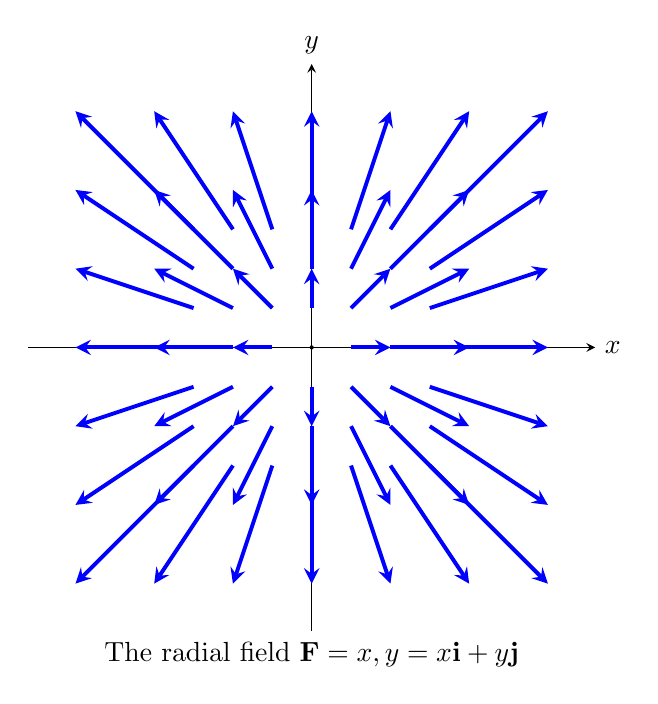
\begin{tikzpicture}[>=stealth, scale=.5]
	%	\draw[dashed, gray!20] (-4,-4) grid (4,4);
	% Draw coordinate axes
	\draw[->] (-7.2,0) -- (7.2,0) node[right] {$x$};
	\draw[->] (0,-7.2) -- (0,7.2) node[above] {$y$};
	% Scaling factor for arrow lengths
	\def\scale{1}
	% Loop over integer grid points
	\foreach \X in {-3,-2,-1,0,1,2,3} {
		\foreach \Y in {-3,-2,-1,0,1,2,3} {
			% Vector field components F = (vx, vy)
			\pgfmathsetmacro{\vx}{\X}
			\pgfmathsetmacro{\vy}{\Y}
			
			% Scaled arrow components (so arrows don't overlap too much)
			\pgfmathsetmacro{\ux}{\scale*\vx}
			\pgfmathsetmacro{\uy}{\scale*\vy}
			
			% Handle the singularity at (0,0)
			\ifnum\X=0
			\ifnum\Y=0
			% Zero vector as a dot
			\fill (0,0) circle (1.5pt);
			\else
			% Non‑zero vector: draw arrow
			\draw[->, line width=.5mm, blue]
			(\X,\Y) -- ++(\ux,\uy);
			\fi
			\else
			\draw[->, line width=.5mm, blue]
			(\X,\Y) -- ++(\ux,\uy);
			\fi
		}
	}
	\node[] at (0,-7.8) {The radial field $\textbf{F}=\gen{x,y}=x\textbf{i}+y\textbf{j}$};
\end{tikzpicture}
\end{minipage}\hfill
\begin{minipage}{.49\textwidth}\centering
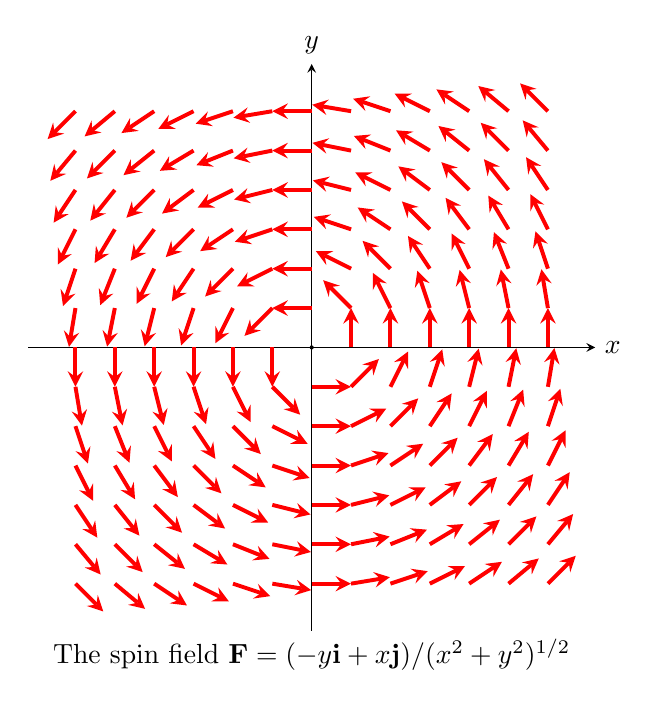
\begin{tikzpicture}[>=stealth, scale=.5]
	%	\draw[dashed, gray!20] (-4,-4) grid (4,4);
	% Axes
	\draw[->] (-7.2,0) -- (7.2,0) node[right] {$x$};
	\draw[->] (0,-7.2) -- (0,7.2) node[above] {$y$};
	% Desired arrow length
	\def\arrowlen{1}	
	% Loop over integer grid points
	\foreach \X in {-6,...,-2,-1,0,1,2,...,6} {
		\foreach \Y in {-6,...,-2,-1,0,1,2,...,6} {
			% Compute radius r = sqrt(x^2+y^2)
			\pgfmathsetmacro{\r}{sqrt(\X*\X + \Y*\Y)}
			
			\ifdim \r pt=0pt
			% At (0,0): singularity
			\fill (0,0) circle (1.5pt);
			\else
			% Compute unit‐tangent components then scale
			\pgfmathsetmacro{\dx}{(-\Y/\r)*\arrowlen}
			\pgfmathsetmacro{\dy}{(\X/\r)*\arrowlen}
			
			% Draw the arrow
			\draw[->, line width=.5mm, red]
			(\X,\Y) -- ++(\dx,\dy);
			\fi
		}
	}
	\node[] at (0,-7.8) {The spin field $\textbf{F}=(-y\textbf{i}+x\textbf{j})/(x^2+y^2)^{1/2}$};
\end{tikzpicture}
\end{minipage}
\end{center}
\end{example*}


\end{document}
